\documentclass[a4paper, 12pt]{article}

\usepackage[utf8]{inputenc}
\usepackage[portuguese,brazil]{babel}
\usepackage{amsmath, amssymb, amsfonts}
\usepackage[a4paper,left=3cm,right=2cm,top=3cm,bottom=2cm]{geometry}
% Caso não queira o 'geometry', pode-se usar:
% \usepackage{a4wide}
\usepackage{tabularx}
\usepackage{graphicx}
\usepackage{pslatex}
\usepackage{indentfirst}
\usepackage{setspace}
\usepackage{verbatim}
\usepackage{hyperref}
\usepackage{float}
\usepackage{algpseudocode,algorithm}
\usepackage[table,xcdraw]{xcolor}

\begin{document}

\thispagestyle{empty}

\begin{minipage}{0.15\linewidth}
\begin{flushleft}

\includegraphics[width=\linewidth]{UFRN}
\end{flushleft}
\end{minipage}\hfill
\begin{minipage}{0.65\linewidth}
\centering Universidade Federal do Rio Grande do Norte\\
Centro de Tecnologia\\
Coordenação de Engenharia de Computação
\end{minipage}\hfill
\begin{minipage}{0.15\linewidth}
\begin{flushright}

\includegraphics[width=0.6\linewidth]{EngComp}
\end{flushright}
\end{minipage}


\vfill

\begin{center}
% \LARGE{\bf Controle embarcado do tipo feedforward/backward para robô com 
% acionamento diferencial, usando encoders magnéticos de baixa resolução}

\Large{Controle embarcado do tipo feedforward/backward para robô com 
acionamento diferencial, usando encoders magnéticos de baixa resolução}
\end{center}

\normalsize
\vfill

\begin{flushleft}
{\bf Aluno(a):} Luís Gabriel Pereira Condados \\
{\bf Orientador acadêmico:}Adelardo Adelino Dantas de Medeiros\\
\end{flushleft}

\vfill

\begin{center}
Natal, RN, \today.
\end{center}

\newpage

\pagenumbering{roman}

\begin{center}
{\bf \Large Agradecimentos}
\end{center}

xxxxx.

\newpage

\tableofcontents

\newpage

% Colocar somente se necessáro...
\listoffigures
\addcontentsline{toc}{section}{Lista de Figuras}

\newpage
% Colocar somente se necessáro...
\listoftables
\addcontentsline{toc}{section}{Lista de Tabelas}

\section{INTRODUÇÃO}

A Equipe Poti de Futebol de Robôs surgiu no Departamento de Engenharia de Computação e Automação da Universidade Federal do Rio Grande do Norte (DCA-UFRN), sendo participante na categoria IEEE Very Small Size Soccer.
\\
Nesse tipo de categoria três robôs de cada time são utilizados de forma cooperativa com o objetivo de fazer o gol. Cada robô possui uma função no jogo, como: o goleiro, o atacante e o defensor, de forma que dependendo da estratégia de jogo eles podem se alternarem para melhor desempenho do time. A arquitetura do sistema do Futebol de Robôs do Time Poti é formada por vários módulos, sendo eles: visão, localização, estratégia, controle e transmissão.\\

O módulo de visão consiste de uma câmera que fotografa o campo com os jogadores e a bola, a taxa de captura da câmera é o fator que limita o tempo de amostragem de todo o sistema, atualmente a equipe utiliza uma taxa de amostragem de $100$ quadros/\emph{frames} por segundo(FPS). O módulo de localização fornece a posição da bola e dos jogadores através das cores que foram predefinidas. O módulo de estratégia é responsável pelo próximo passe que os robôs deverão executar, a partir das imagens atuais. O módulo de controle é responsável por converte as referências de posição e orientação, definidas pela estratégia, em sinais que correspondem as velocidades que devem ser aplicadas nas rodas direita e esquerda de cada robô e o módulo de transmissão envia esse sinal para os robôs.\\

O objetivo deste trabalho foi projetar e implementar um novo sistema de \textit{Hardware} e \textit{Firmware} para esses robôs. Os robôs antes deste trabalho possuíam um controlador da \emph{Atmega} de 32\emph{bits single core} usado em um módulo de desenvolvimento rápido (\emph{Arduino Nano}), um módulo \\emph{Bluetooth}, \emph{Drivers} motores e não possuía controle embarcado, ou seja, os sinais de controle dos motores direito e esquerdo direto eram provenientes diretamente do módulo de transmissão.\\

O novo \textit{Hardware}  conta com um microcontrolador dual core de 32\emph{bits} (ESP32) e \textit{Encoders} magnéticos de baixa resolução. Foi embarcado  nesse microcontrolador um controle de velocidade angular do tipo  \textit{FeedForward}/\textit{Backward}(PID), que deve atuar no par de motores dos robôs de  forma a controlar suas velocidades bem como reduzir as assimetrias entre  os motores direito e esquerdo.\\

Usando a interface \textit{Bluetooth} presente no microcontrolador, foi criado um  protocolo simples de comunicação para realizar operações de telemetria e telecomando nos robôs. O \textit{Firmware} opera utilizando os dois núcleos  executando tarefas distintas: um núcleo é responsável pela comunicação  com o servidor, por meio do \textit{Bluetooth} e do protocolo criado, bem como  por tratar as interrupções geradas pelos \textit{Encoders} rotativos magnéticos;  já o outro núcleo executa a rotina de controle, com um período de amostragem de pelo menos $5$ms, para operar em uma frequência de pelo menos duas vezes mais rápido que o sistema que está rodando no \emph{host}, que como já mencionado trabalha até à $100$fps ($10$ms).\\

% resolução do encoder: 3 pulsos por revolução ou
% 6 pulsos se contar os dois canais ou
% 12 bordas de subida e descida nos dois canais por revolução
Para medir a velocidade de rotação, foram utilizados \textit{Encoders} magnéticos  rotativos, com resolução de $3$ pulsos por canal por revolução do eixo do motor. Para diminuir a  incerteza na estimativa da velocidade, é aplicado um filtro de \textit{Kalman},  considerando a planta (motores) como um sistema de primeira ordem. Os  parâmetros da planta (constante de tempo, zona morta e ganho PWM x  Velocidade angular) são estimados/calculados por mínimos quadrados na  rotina de calibração presente no \textit{Firmware}, sendo em seguida utilizados  para determinar os parâmetros do controlador.

% Organização do trabalho
% Este trabalhado é organizado da seguinte maneira: O Capítulo 1 corresponde à introdução do trabalho, por meio da qual é feita uma contextualização do problema e a proposta de solução para o mesmo; o capítulo 2 traz a fundamentação teórica utilizada para o desenvolvimento deste trabalho; no capítulo 3, os objetivos gerais e específicos são abordados; no capítulo 4 são apresentados os materiais e métodos utilizados para implementação do sistema; o capítulo 5 contém os resultados e discussões em que podem ser observadas as telas do sistema proposto; no capítulo 6 as conclusões deste trabalho são levadas em consideração, assim como sugestões de trabalhos futuros.
\section{REFERENCIAL TEÓRICO}
Nesta seção será apresentado os principais conceitos utilizados neste trabalho, como a modelagem do motor de corrente contínua utilizada; Filtro de \emph{Kalman}; Introdução à Teórica de Controle; Comunicação \emph{Bluetooth}, entre outras coisos conceitos.
%************************************************************************** 
\subsection{Motor de Corrente Contínua}
% Introduzir o que funcionamento básico de um motor CC
% deixar claro qual o tipo será apresentado/utilizado no trabalho (motor CC de campo magnético fixo e com "escova")
Como o próprio nome indica, os motores CC são acionados por uma fonte de corrente contínua. São motores que possuem ímãs permanentes ou então têm campo e armadura. Esse tipo de motor é amplamente utilizado em diversas aplicações.

Ele é constituído basicamente pelo enrolamento de armadura, enrolamento de campo, comutador e as escovas, onde:

\begin{itemize}
    \item Enrolamento de armadura: é localizado na parte giratória do motor de CC (rotor) que é responsável por produzir o torque que o movimenta, bem como a tensão de saída quando em modo de gerador.
    
    \item Enrolamento de campo: parte fixa responsável pelo fluxo magnético constante que irá atravessar a armadura. 
    
    \item Comutador: Possui a função de manter a corrente da armadura circulando no mesmo sentido, fazendo com que o torque mantenha seu sentido para uma tensão de entrada constante.
    
    \item Escovas: é por onde acontece o contato do enrolamento de armadura com a fonte de alimentação.
\end{itemize}


As máquinas de corrente contínua são bastante utilizadas em sistema de controle em razão do seu comportamento essencialmente linear [apostilha:modelagem]. O diagrama esquemático de uma máquina (motor ou gerador) CC é mostrado na figura \ref{fig:modelo_motor_dc}. O enrolamento de campo tem resistência $R_f$ e indutância $L_f$ e o enrolamento de armadura tem resistência $R_a$ e indutância $L_a$. As correntes e tensões nos enrolamentos de campo e de armadura $i_f$, $v_f$, $i_a$ e $v_a$, respectivamente. A tensão induzida na armadura é $v_g$. O torque e a velocidade angular no eixo do rotor são $\tau$ e $\omega$, respectivamente.

A tensão induzida no enrolamento de armadura é dada por:

\begin{equation}
    v_g = K_{1}\phi\omega
\end{equation}

E o torque é dado por:

\begin{equation}
    \tau = K_{1} \phi i_a 
\end{equation}

Onde $K_1$ é um parâmetro determinado pela estrutura física da máquina e $\phi$ é o fluxo magnético. Supondo que a máquina esteja operando na zona linear (ou seja, que o núcleo não esteja saturado), o fluxo é dado pela equação:

\begin{equation}
    \phi = K_{2}i_f
\end{equation}

Onde $K_2$ é uma constante e depende das características magnéticas do núcleo e do enrolamento de campo.

Motores geram potência mecânica, de forma que a velocidade de rotação $\omega$ é o sinal de saída e a tensão $v_a$ aplicada é o sinal de entrada. 

\begin{figure}[H]
    \centering
    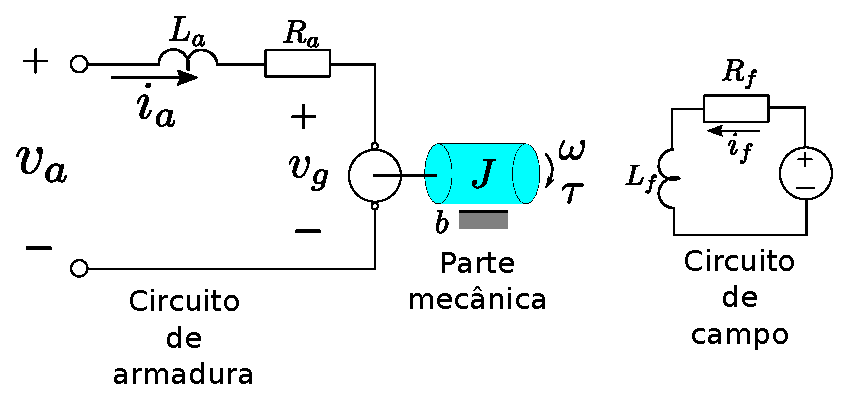
\includegraphics[width=0.5\textwidth]{imagens/ilustracoes/esquematico_motor_dc.eps}
    \caption{Diagrama esquemático de um motor CC.}
    \label{fig:modelo_motor_dc}
\end{figure}


A figura \ref{fig:modelo_motor_dc} apresenta o diagrama esquemático para um motor de corrente contínua (CC) controlado pela armadura, ou seja, o sinal de entrada é a tensão aplicada na armadura ($v_a$). Nesse diagrama a carga está sendo modelada por um momento de inércia $J$ e um atrito viscoso de coeficiente $b$.

\begin{align*}
    v_g &= K_{1}\phi\omega= K_{1}K_{2}i_{f}\omega = K_{m}\omega\\
    \tau &= K_{1} \phi i_{a}= K_{1} K_{2}i_{f} i_{a} = K_{m}i_{a}
\end{align*}

A constante $K_{m}$ é conhecida como a constante do motor. Devido a relação apresentada anterior é possível modelar o circuito equivalente do motor CC como na imagem \ref{fig:eq_eletrico_motorcc}.
% figura retirada do livro texto da disciplina de modelagem.
\begin{figure}[H]
    \centering
    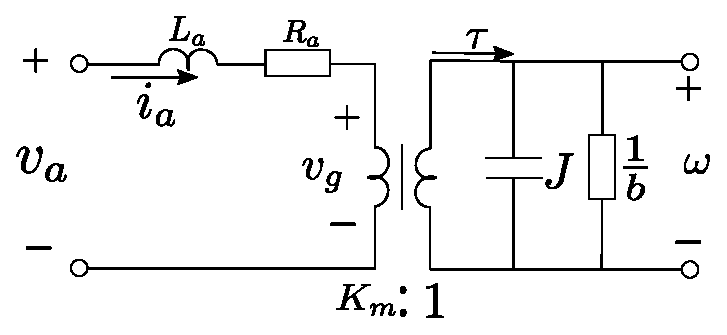
\includegraphics[width=0.6\textwidth]{imagens/ilustracoes/circuito_equivalente_motor_cc.eps}
    \caption{Equivalente elétrico de um motor CC}
    \label{fig:eq_eletrico_motorcc}
\end{figure}

Do circuito da figura \ref{fig:eq_eletrico_motorcc} extrai-se a seguinte função de transferência:

\begin{equation*}
    \frac{\Omega(s)}{V_a(s)} = \frac{K_m}{JL_{a}s^2 + \left(JR_a + BL_a \right)s + BR_a + K_{m}^2} \left[\frac{ rad.s^{-1}}{V}  \right]
\end{equation*}

Caso a impedância da armadura seja desprezada $(L_a \xrightarrow{} 0)$:

\begin{equation}
    \frac{\Omega(s)}{V_{a}(s)} = \frac{K_m}{JR_{a}s + BR_{a} + K_{m}^2} = \frac{K}{T_{m}s + 1} \left[\frac{ rad.s^{-1}}{V}  \right]
    \label{eq:motor_transf_func}
\end{equation}

Portando, caso a impedância da armadura seja desprezada, a função de transferência do motor que relacionada a velocidade angular com a tensão de entrada se comporta como um sistema de primeira ordem. A maior dificuldade encontrada ao se controlar motores CC é a amplitude elevada da corrente de armadura, o que requer a utilização de sinal $v_a$ de entrada fornecido por uma fonte de alta potência [apostilha].
\subsection{Sistemas de Controle}

O controle automático é um componente importante e intrínseco em sistemas de veículos espaciais, sistemas robóticos, modernos sistemas de manufatura e quaisquer operações industriais que envolvam o controle de temperatura, pressão, umidade, viscosidade, vazão etc [Okata:Eng.Controle Moderno]. Um problema de controle consiste em determinar uma forma de afetar um dado sistema físico de modo que seu comportamento atenda às especificações de desempenho previamente estabelecidas. Como, normalmente, não é possível alterar a estrutura funcional do sistema físico em questão, a satisfação das especificações de desempenho é atingida mediante o projeto e implementação de controladores (compensadores) [apostilha]. Algumas \textbf{definições/terminologias} comuns no contexto de sistema de controle são apresentadas a seguir.

%[Okata:Eng.Controle Moderno]
Segundo [?].
\textbf{Sinal de controle ou variável manipulada.} Como o próprio nome indica, é a grandeza controlada/manipulada. É o sinal que é modificado pelo controlador, de modo a afetar a variável que se está controlando. Geralmente o sinal de controle é a saída do sistema (entrada da planta).\\

\textbf{Planta.} Uma planta pode ser um equipamento, parte de um equipamento ou um conjunto que funciona de maneira integrada, com o objetivo de realizar uma determinada tarefa. Pode ser qualquer mecanismo/objetivo físico a ser controlado (como por exemplo, um motor, um reator ou qualquer componente mecânico no geral).

\textbf{Processos.} Caracteriza-se por ser qualquer operação com um desenvolvimento por mudanças graduais e progressivas que se sucedem de forma a conduzir um resultado ou uma determinada finalidade.

\textbf{Sistemas.} É uma combinação de vários componentes que trabalham em conjunto para atingir um determinado objetivo. O conceito pode ser aplicado tanto para fenômenos físicos quanto para fenômenos abstratos.

\textbf{Distúrbios.} É uma interferência (sinal adverso) que influência na saída de um sistema. Pode ocorrer internamente ao sistema quando externamente.


\textbf{Controle.} Ação por meio da qual se manipula um sistema físico visando fazer com que este atenda um determinado conjunto de especificações determinadas a priori.

\textbf{Controlador.} Dispositivo utilizado para realizar o controle de um sistema físico.



\textbf{Sistema de controle em malha aberta (\emph{Feedforward}).} Sistema de controle que não possui a entrada influenciada pela saída do sistema. Isso quer dizer que, o sinal de saída não é medido nem realimentado para comparação com a entrada (Ver Figura \ref{fig:ilustracao_sistema_malha_aberta}). Devido a natureza desse tipo de controle, a entrada de referência é mapeada para uma saída fixa do controlador. Dessa maneira, a precisão do sistema depende de uma calibração para melhor ajustar/mapear a referência em um determinado sinal de controle.

\begin{figure}[H]
    \centering
    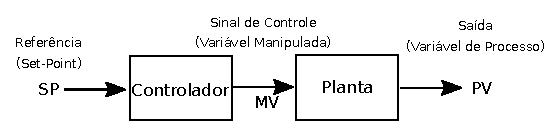
\includegraphics[width=0.8\textwidth]{imagens/ilustracoes/diagrama_sistema_malha_aberta.eps}
    \caption{Diagrama de exemplificação de sistema de controle em malha aberta.}
    \label{fig:ilustracao_sistema_malha_aberta}
\end{figure}

\textbf{Sistema de controle em malha fechada.} Difere essencialmente do em malha aberta, pois neste tipo a entrada do controlador é influenciada pela saída da planta (variável de processo) (Ver Figura \ref{fig:ilustracao_sistema_malha_fechada}). Esse tipo de sistema de controle também é denominado de controle com realimentação (controle com \emph{Feedback}). A relação entre a saída e a entrada de referência se dar por meio da comparação entre elas, utilizando a diferença como meio de controle.

\begin{figure}[H]
    \centering
    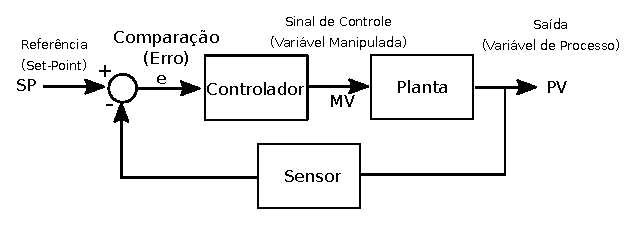
\includegraphics[width=0.8\textwidth]{imagens/ilustracoes/diagrama_sistema_malha_fechada.eps}
    \caption{Diagrama de exemplificação de sistema de controle em malha fechada.}
    \label{fig:ilustracao_sistema_malha_fechada}
\end{figure}


Segundo [Okata] as principais vantagens do sistema de controle em malha aberta são:
\begin{enumerate}
    \item São de fácil construção/implementação e fácil manutenção.
    \item Não apresentam problemas de estabilidade.
    \item São mais adequados em situações em que a medição precisa da saída é um problema.
\end{enumerate}

E algumas desvantagens:

\begin{enumerate}
    \item Distúrbios e mudanças na calibração causam erros, e a saída pode apresentar diferenças
    em relação ao padrão desejado.
    \item Para que a saída mantenha a qualidade requerida, é necessária uma regulagem periódica.
\end{enumerate}


\subsubsection{Controlador PID}
% Controlador PID
% Controlador malha aberta Feedforward
Um controlador clássico do tipo \emph{Feedback} e que ainda é muito utilizado é o controlador proporcional Integral derivativo (PID). Como o próprio nome indica, esse tipo de controlador une as ações derivativa, integral e proporcional. A ação proporcional faz com que o erro diminua e influência no tempo de resposta do sistema, a ação integral elimina o erro de regime e a ação derivativa influência no tempo de resposta do sistema, por meio da antecipação do erro.

Definindo-se os seguintes sinais no tempo: $u(t)$ como sinal de saída (sinal de controle) e $e(t)$ como o erro entre a referência e o valor atual da saída da planta, o controlador pode ser definido como:

\begin{equation}
    u(t) = K_{p}e(t) + K_{i} \int^{t}_{0}e(\tau)d\tau + K_{d}\frac{d e(t)}{dt}
\end{equation}

Aplicando a transformada \emph{Laplace} temos,

\begin{equation}
    \frac{U(s)}{E(s)} = K_{p} + \frac{K_{i}}{s} + K_{d}s
\end{equation}

Sendo,

\begin{itemize}
    \item $K_p$: O ganho proporcional.
    \item $K_i$: Ganho integral.
    \item $K_d$: Ganho derivativo.
    \item $s$: Frequência complexa.
\end{itemize}

Esse tipo de controlador pode ser utilizado em mais três formas básicas além do padrão PID: Controle Proporcional (P). Apenas a ação proporcional; Controle Proporcional Integral (PI) e Controle Proporcional Derivativo (PD).

\begin{figure}[H]
    \centering
    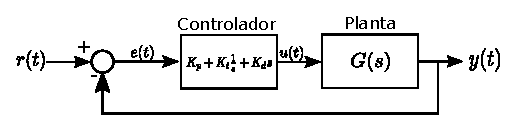
\includegraphics[width=\textwidth]{imagens/ilustracoes/diagrama_controlador_PID.eps}
    \caption{Diagrama de um sistema controlado por PID.}
    \label{fig:diagrama_controlador_PID}
\end{figure}

A Figura \ref{fig:diagrama_controlador_PID} ilustra em diagrama de blocos o uso do controlador PID. Onde $r(t)$ é o sinal de referência (\emph{set-point}), $y(t)$ é a saída da planta e $G(s) = Y(s)/U(s)$ é a função de transferência da panta.

\begin{figure}[H]
    \centering
    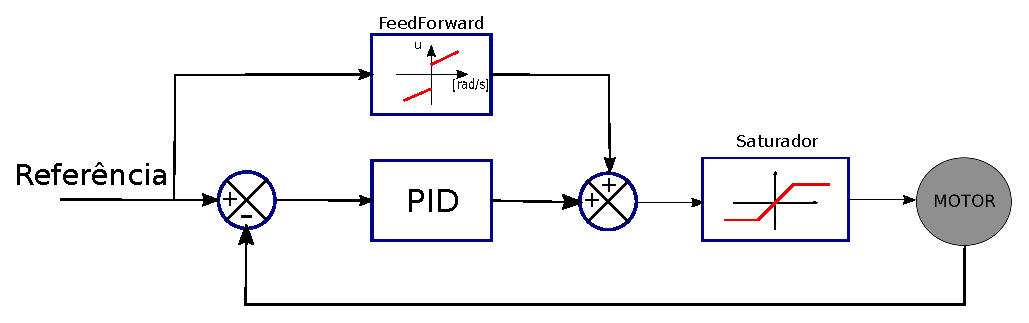
\includegraphics[width=\textwidth]{imagens/ilustracoes/sistema_de_controle_completo.eps}
    \caption{Diagrama de um sistema de controle \textit{Feedforward} + \textit{Backward}}
    \label{fig:diagrama_sistema_de_controle_feedforward_backward}
\end{figure}

\subsubsection{Sistemas de Primeira Ordem}

Um sistema de primeira ordem apresenta a seguinte forma genérica:

\begin{equation}
    T\dot{y} + y = Ku
\end{equation}

E em \emph{Laplace} com a seguinte função de transferência,

\begin{equation}
    G(s) = \frac{K}{Ts + 1}
\end{equation}

E sua resposta no tempo para uma entrada do tipo degrau unitário ($u(t) = 1 \xrightarrow{\mathscr{L}} U(s) = 1/s$),

\begin{equation}
    y(t) = K \left(1 - e^{-t/T} \right)
\end{equation}

Sendo $K$ o ganho do sistema e a constante $T$ é conhecida como constante de tempo do sistema e $T > 0$. A Figura \ref{fig:saida_sistema_primeira_ordem_no_tempo} ilustra o comportamento no tempo de um sistema de primeira ordem e a influência da constante de tempo $T$ na resposta do sistema.

\begin{figure}[H]
    \centering
    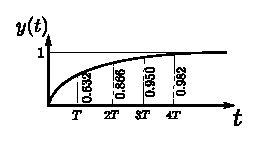
\includegraphics[width=0.7\textwidth]{imagens/ilustracoes/resposta_no_tempo_sistema_primeira_ordem.eps}
    \caption{Resposta no tempo ao degrau unitário de um sistema de primeira ordem com ganho unitário e contante de tempo $T$.}
    \label{fig:saida_sistema_primeira_ordem_no_tempo}
\end{figure}

% O erro de regime é a diferença entre os sinais de entrada e de saída na região de regime da resposta. Ou seja, $t \xrightarrow{} \infty$.
\input{tex/referenciais_teoricos/sistemas_primeira_ordem}
\subsection{Mínimos Quadrados}
\subsection{Filtro de Kalman}
% Introdução ao filtro de Kalman

Modelo do sistema:
\begin{equation}
\textbf{x}_k = F_x x_{k-1} + B_k u_k + w_k; w_k \sim N(0, Q_k)
\end{equation}

Modelo da medição:
\begin{equation}
z_k = H_k x_k + v_k; v_k \sim N(0, R_k)
\end{equation}

Predição:
\begin{align*}
    \check{x}_k &= F_k \hat{x}_{k-1} + B_k u_k\\
    \check{P}_k &= F_k \hat{P}_{k-1} F^T_k + Q_k
\end{align*}

Atualização:
\begin{align*}
    K_k &= \check{P}_k H^T \left( H_k \check{P}_k H^T_k + R_k\right)^{-1}\\
    \hat{x}_k &= \check{x}_k + K_k\left( z_k - H_k \check{x}_k \right)\\
    \hat{P}_k &= \left(I - KH_k \right)\check{P}_k
\end{align*}
\subsection{\textit{Encoders} Rotativos Incrementais}
% Referencias:
% https://www.roboticsbusinessreview.com/news/differences-between-encoder-resolution-accuracy-and-precision/
% https://www.newtoncbraga.com.br/index.php/como-funciona/5454-mec128
% [Speed Measumment Using Rotary Encoders for High Performance ac Drives]
% [Speed Measurement Algorithms for Low-Resolution Incremental Encoder Equipped Drives: a Comparative Analysis]
% [A Simple Speed Feedback System for Low Speed DC Motor Control in Robotic Applications]
% [An Embedded System for Position and Speed Measurement Adopting Incremental Encoders]

% FALAR SOBRE O FUNCIONAMENTO BASICO
% CITAR OS DIFERENTES TIPOS
% FALAR DO GRAY CODE
% FALAR DO ERRO DE QUANTIZAÇÃO

As saídas de um \emph{Encoder} incremental são, normalmente, duas ondas quadradas defasadas em $90^\circ$ uma da outra (em quadratura). Essa diferença de fase nos permite medir o sentido de rotação. Abordagens mais eficientes de leitura desses sensores é por meio da detecção das bordas dessas ondas, pois isso permite quadruplicar o número de pulsos por revolução (NPR) [?]. Existem dois métodos básicos para se realizar a medição da velocidade por meio desses sensores, são eles: \textbf{frequencímetro} e \textbf{periodímetro}. 

Na medição por frequência (\textbf{frequencímetro}), conta-se o número de pulsos que ocorreram em um determinado período de tempo fixo. Com isso a velocidade pode ser obtida pela seguinte aproximação:

\begin{equation}
    \omega = \frac{d\theta}{dt} \cong \frac{\Delta{\theta}}{T} \cong \frac{2 \pi \Delta{N}}{N_{PR}T}[rad.s^{-1}] \xrightarrow{} \frac{60 \Delta{N}}{N_{PR} T} [RPM]
\end{equation}

Sendo $N_{PR}$ o número de pulsos por revolução e $\Delta{N}$ é o número de pulsos que aconteceram dentro da janela de tempo $T$. Existe um erro de quantização nesse método de leitura devido a variação de ângulo medida ser sempre um múltiplo inteiro de $ 2\pi/N_{PR}$. O erro de quantização $\Delta{\omega}$ pode ser modelado pela seguinte equação:

\begin{equation}
    \Delta{\omega} = \frac{2\pi}{N_{p}T}[rad.s^{-1}] \xrightarrow{} \frac{60}{N_{PR}T}[RPM]
    \label{eq:erro_de_quantizacao_frequencimetro}
\end{equation}

\begin{figure}[H]
    \centering
    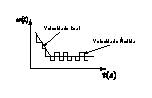
\includegraphics[width=0.5\textwidth]{imagens/ilustracoes/ilustracao_erro_de_quantizacao.eps}
    \caption{Ilustração do erro de quantização na medição de velocidade de rotação.}
    \label{fig:ilustracao_erro_quantizacao}
\end{figure}

A Figura \ref{fig:ilustracao_erro_quantizacao} ilustra um exemplo de medição de velocidade com erro de quantização.\\

Nota-se pela Equação \ref{eq:erro_de_quantizacao_frequencimetro} que o erro de quantização para a medição por frequência decresce com o aumento do número de pulsos por revolução e/ou com o aumento da janela de tempo ($T$), porém o aumento do período de observação acrescenta um atraso na medição da velocidade. O erro relativo à velocidade pode ser descrito como a seguir:

\begin{equation}
    e_{\omega}\% = \frac{2\pi}{\omega N_{PR} T}.100
    \label{eq:erro_relativo_quantizacao_frequencimetro}
\end{equation}

Pela Equação \ref{eq:erro_relativo_quantizacao_frequencimetro} observa-se que o erro relativo decresce conforme a velocidade $\omega$ aumenta, ou seja, o erro de quantização será mais significante para baixas velocidades.\\

O outro método de leitura dos \emph{Encoders} incrementais é por medição de intervalos de tempo de um mesmo pulso (\textbf{periodímetro}) (ver Figura \ref{fig:ilustracao_periodimetro}). A seguinte formulação pode ser obtida considerando a velocidade do motor constante e sem levar em conta o sentido de giro:

\begin{equation}
    \omega = \frac{d\theta}{dt} \cong \frac{\Delta{\theta}}{nT_{hf}} \cong \frac{2\pi}{N_{PR} n T_{hf}} [rad.s^{-1}] \xrightarrow{} \frac{60}{N_{PR} n T_{hf}} [RPM]
    \label{eq:omega_periodimetro}
\end{equation}

O período entre pulsos será:

\begin{equation}
    T_{\omega}(\omega) = \frac{2\pi}{N_{p}\omega} [s]
\end{equation}

Uma aproximação para o pior caso do erro de quantização relativo a velocidade é apresentado a seguir [?]:

\begin{equation}
    e_{\omega}\% = \frac{T_{hf}}{ \frac{2\pi}{N_{PR} \omega} - T_{hf} }.100 \cong \frac{\omega N_{PR} T_{hf}}{2\pi}.100
    \label{eq:erro_quantizacao_periodimetro}
\end{equation}

A Equação \ref{eq:erro_quantizacao_periodimetro} mostra que o erro é diretamente proporcional à velocidade e a quantidade de pulsos por revolução ($N_{PR}$) e decresce com o aumento da frequência do contador de alta frequência (diminuição de $T_{hf}$).


\begin{figure}[H]
    \centering
    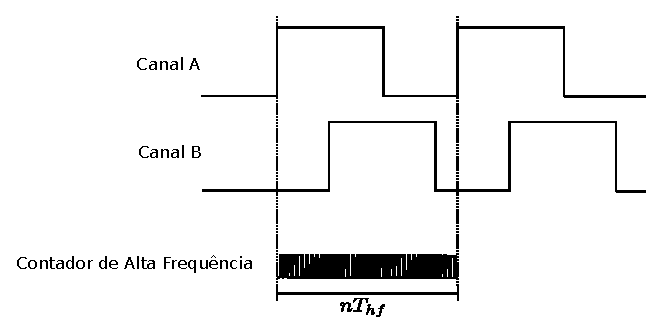
\includegraphics[width=0.5\textwidth]{imagens/ilustracoes/ilustracao_medicao_encoder_por_periodo.eps}
    \caption{Ilustração de leitura de \emph{Encoder} periódica.}
    \label{fig:ilustracao_periodimetro}
\end{figure}

Já para se obter o \textbf{sentido da velocidade $\omega$} é necessário fazer uso do padrão binário gerado pelas bordas dos sinais em quadratura. A Figura \ref{fig:cw_signal} ilustrado os sinais em quadratura para uma rotação no sentido horário e destaca o padrão binário gerado nas bordas. A Figura \ref{fig:ccw_signal} ilustra os sinais no sentido anti-horário. O padrão de dois bits é apresentado na Tabela \ref{tab:tabela_simple_code}. \\

\begin{figure}[H]
    \centering
    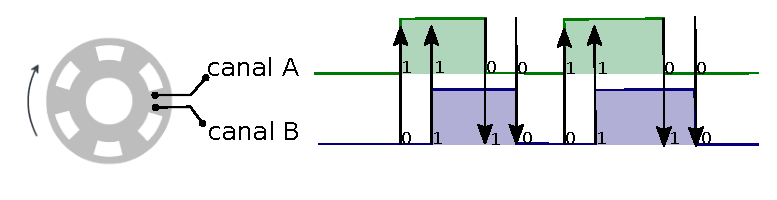
\includegraphics[width=0.7\textwidth]{imagens/ilustracoes/sinal_enquadratura_sentido_CW.eps}
    \caption{Sinal em quadratura para rotação no sentido horário.}
    \label{fig:cw_signal}
\end{figure}

\begin{figure}[H]
    \centering
    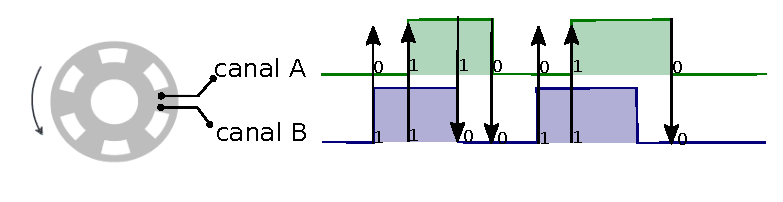
\includegraphics[width=0.7\textwidth]{imagens/ilustracoes/sinal_enquadratura_sentido_CCW.eps}
    \caption{Sinal em quadratura para rotação no sentido anti-horário.}
    \label{fig:ccw_signal}
\end{figure}

% Please add the following required packages to your document preamble:
% \usepackage{graphicx}
\begin{table}[H]
\centering
\resizebox{0.5\textwidth}{!}{%
\begin{tabular}{cc|cc}
\multicolumn{2}{c|}{\textbf{\begin{tabular}[c]{@{}c@{}}Sentido\\     Horário\end{tabular}}} &
  \multicolumn{2}{c}{\textbf{\begin{tabular}[c]{@{}c@{}}Sentido\\ Anti-Horário\end{tabular}}} \\ \hline
\textbf{A} & \textbf{B} & \textbf{A} & \textbf{B} \\
1          & 0          & 1          & 0          \\
0          & 1          & 0          & 1         
\end{tabular}%
}
\caption{Código de 2 bits para identificar o sentido de rotação.}
\label{tab:tabela_simple_code}
\end{table}


\begin{comment}
% Speed Measumment Using Rotary Encoders
% for High Performance ac Drives

SPEED MEASUREMENT USING A PERIODIMETER

If we use a periodimeter, we will get the speed not by counting pulses from the encoder, but by counting a high frequency (HF) clock

Let $\alpha_p$ be the corresponding angle to the higher part of an encoder pulse (half of its period), t the period of the HF clock, and n the number of HF pulses arrived at the HF counter. Then, the time spent on an encoder pulse, $T_e$ is:

\begin{equation}
    T_e = n t
\end{equation}

Rotor speed can be obtained as:

\begin{equation}
    \omega_{rotor} = \frac{\alpha_p}{T_e}
\end{equation}

As with the frequencimeter, here also there is a quantization error because of the time T,, which will be always an integer multiple of t With a fixed HFclock frequency, this error will increase as n decreases, that is, as the encoder rotates faster, but it provides accurate measurements at lower speeds. Because the variable with quantization noise is now in the denominator, its effects are much more important than in the frequencimeter.

An additional advantage at low speed is that, as it only needs one pulse to get the speed, the delay is minimal, which is very important at lower speeds.

It also possible to use quadruple frequency. Of course, this reduces the precision, and therefore the maximum velocity where this method is suitable, but also, and this is much more important, it reduces the delay obtaining the velocity when the motor works at low speed. Nevertheless, this method produces stability problems in the zero speed cross. Figure 8 shows an inversion with two possible situations in the encoder output signals. Supposing that there is no quadruple frecuency, and PHASE A controls the HF counter, we see that at the encoder pulse end, the counter has a wrong value, because about half of the HF pulses arrived on each direction of rotation.

The accuracy of the periodimeter is, more than the frequencimeter, related to the accuracy of the encoder, which in general depends on the errors in the radial grating, and the eccentricity of the graduated disk to the bearing.

% Speed Measurement Algorithms for
% Low-Resolution Incremental Encoder Equipped
% Drives: a Comparative Analysis


At very low speed the number of high frequency pulses can be extremely high and saturation of the digital timer employed for measurement can occur. Also a speed sample is not available each speed control period, needing an adaptation of the control parameters. In that situation, the quadrature decoding of the encoder pulses can be exploited in order to reduce the width of the measuring window by a factor of four or a reduction of the frequency of the timer can be considered.

The former solution allows to reduce the speed sampling period and improve the control performance of the drive, but makes the measuring system more sensitive to sensor nonidealities, including variations in the transition locations from their nominal values and phasing errors between encoder channels. When low-cost and low-resolution sensors are employed, nonidealities play the major role in the determination of period measuring errors and has to be carefully analysed in drive design phase. The latter solution needs to switch on-line the frequency of the timer and adapt the coeffients of the equations above.

The implementation of the period measuring method is also straightforward as it requires a simple timer capture unit, commonly found inside recent microcontrollers.

% A Simple Speed Feedback System for Low Speed
% DC Motor Control in Robotic Applications

The relationship between the measured frequency using PIC microcontroller and the percentage error is shown in Fig. 2. The percentage error is given as:

\begin{equation}
    e\% = \frac{F_m - F_a}{F_a}.100
\end{equation}

where F m and F a denote the measured and actual frequencies. It is observed that as the frequency increases, the error in the frequency measured from PIC increases linearly, that is, there is a linear relationship between error and frequency.

\end{comment}
\subsection{Bluetooth}
% Breve introdução à historia do bluetooth e utilidade
% destacar: custo energético, velocidade de operação, robustez a interferências
A  tecnologia \emph{Bluetooth}  suporta várias opções de topologia, incluindo conexões simples ponto a ponto. Operando na faixa de frequência industrial, científica e médica de $2,4$ GHz, a tecnologia \emph{Bluetooth} suporta várias opções de rádio.

O rádio \emph{Bluetooth} BR/EDR opera com baixo consumo de energia e também utiliza uma abordagem robusta de \textit{Adaptive Frequency Hopping}, transmitindo dados por $79$ canais. O \textit{Bluetooth} BR/EDR inclui várias opções de \textit{PHY} que suportam taxas de dados de $1$ Mb a $3$ Mb e suporta vários níveis de energia, de $1$mW a $100$ mW, além de várias opções de segurança.

% aprofundar mais? 
\subsection{Modulação por Largura de Pulso}
% Resumo sobre PWM
\section{MATERIAIS E MÉTODOS}
Como já mencionado, o objetivo básico do projeto foi projetar os robôs da equipe de futebol de robôs do laboratório de robótica do DCA, sendo assim os robôs devem ter suas dimensões limitadas a um cubo de $75$mm de aresta, essa foi umas das principais restrições levada em conta para o projeto eletrônico dos robôs, além do fator econômico.  A parte estrutural do robô não será abordada neste trabalho, mas sim a parte eletrônica e de software.

\subsection{Componentes}
% Listas os componentes utilizados na montagem e mostrar algumas de suas
% principais características e sua finalidade no projeto
% mostrar o diagrama eletrônico
% Falar um pouco sobre o funcionamento dos sensores
% Falar como foi implementado a leitura, as otimizações feitas
São quatro o número de componentes básicos que compõem os robôs presentes neste trabalho, sendo eles: um par de atuadores (motor direito e esquerdo), um par de sensores de rotação (\textit{Encoder}s magnéticos), um driver motor multicanal, um microcontrolador e bateria recarregável. Devido as características dos componentes escolhidos para o projeto, apenas estes quatro tipos foram suficiente para compor a eletrônica do robô de forma a respeitar as restrições dimensionais, realizar o controle feedforward/backward de forma eficiência e com um bom período de amostragem e baixo gasto energético, além de um baixo custo financeiro.

A seguir serão apresentados mais detalhes dos componentes supracitados.

% 30:1 Micro Metal Gearmotor HP 6V with Extended Motor Shaft
\begin{figure}[H]
    \centering
    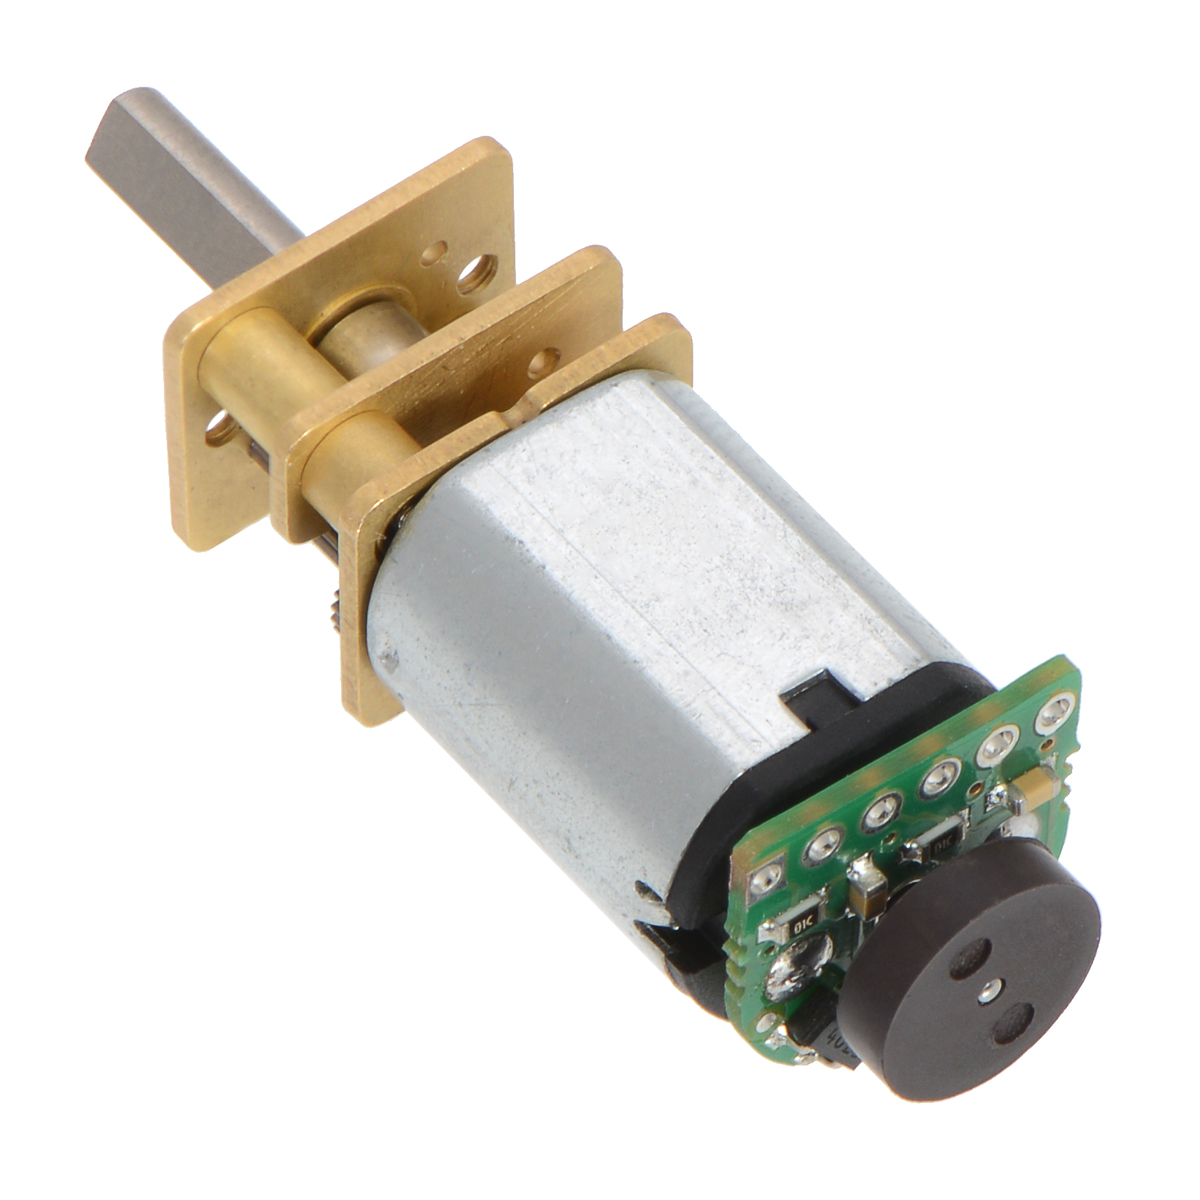
\includegraphics[width=3cm]{imagens/eletronica/motor_com_encoder.jpg}
    \caption{Micro Motor de 6V com caixa de redução de 30:1 e \textit{Encoder} magnético.}
    \label{fig:motor_com_encoder}
\end{figure}

A figura \ref{fig:motor_com_encoder} mostra o motor escolhido já com o \textit{Encoder} magnético colocado em seu eixo estendido (placa de circuito impresso com um Imã natural em forma de disco), esse é um micro motor de $6$V com uma caixa de redução de $\approx 30:1$ da \textit{Pololu}[?].

\begin{figure}[H]
    \centering
    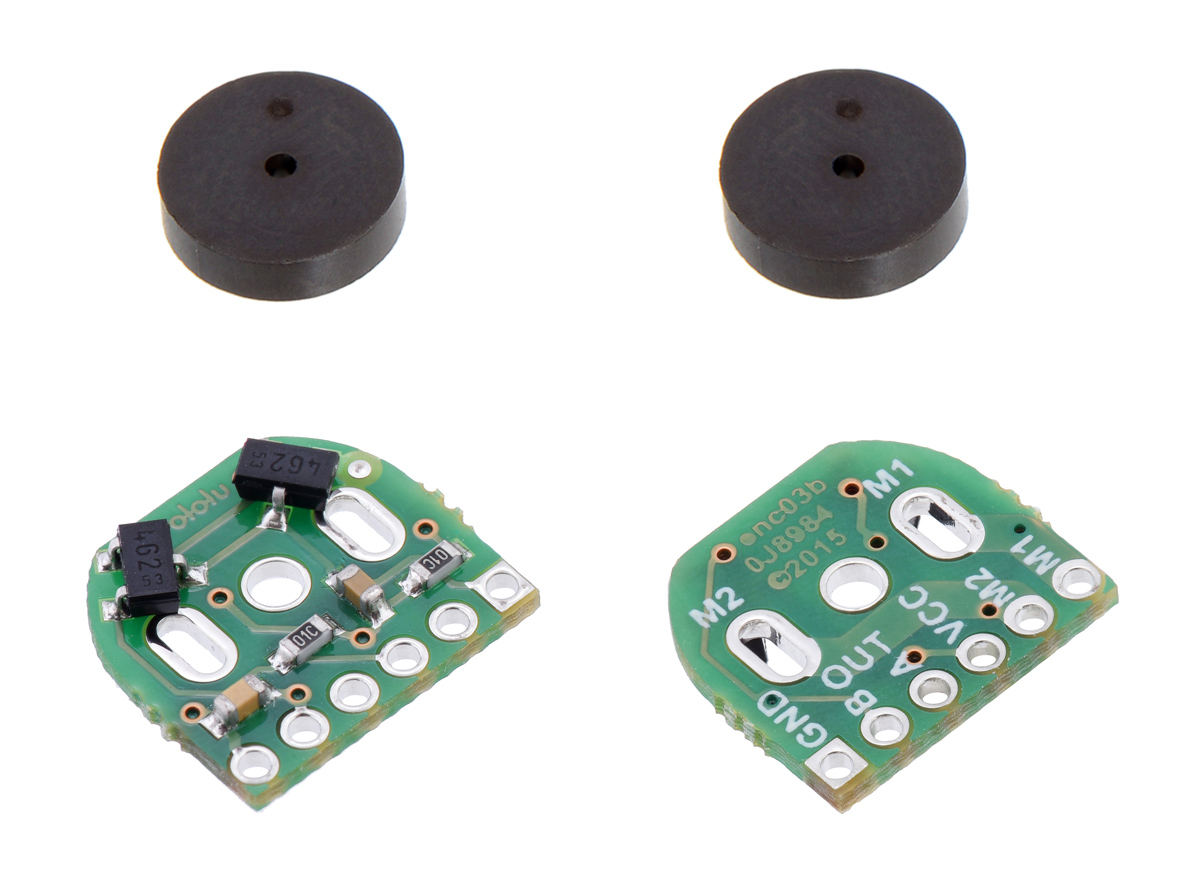
\includegraphics[width=5cm]{imagens/eletronica/encoder_frente_verso.jpg}
    \caption{Par de Encoders Magnéticos de $12$ pulsos por revolução ($12$CPR)}
    \label{fig:encoder}
\end{figure}

\begin{figure}[H]
    \centering
    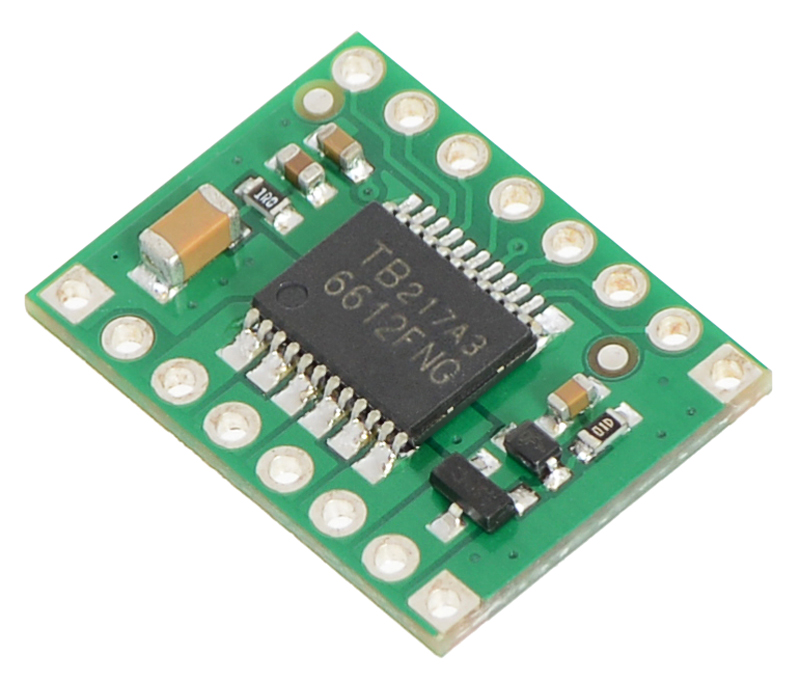
\includegraphics[width=3cm]{imagens/eletronica/driver.jpg}
    \caption{\textit{Driver} Motor TB6612FNG.}
    \label{fig:driver_motor}
\end{figure}

\begin{figure}[H]
    \centering
    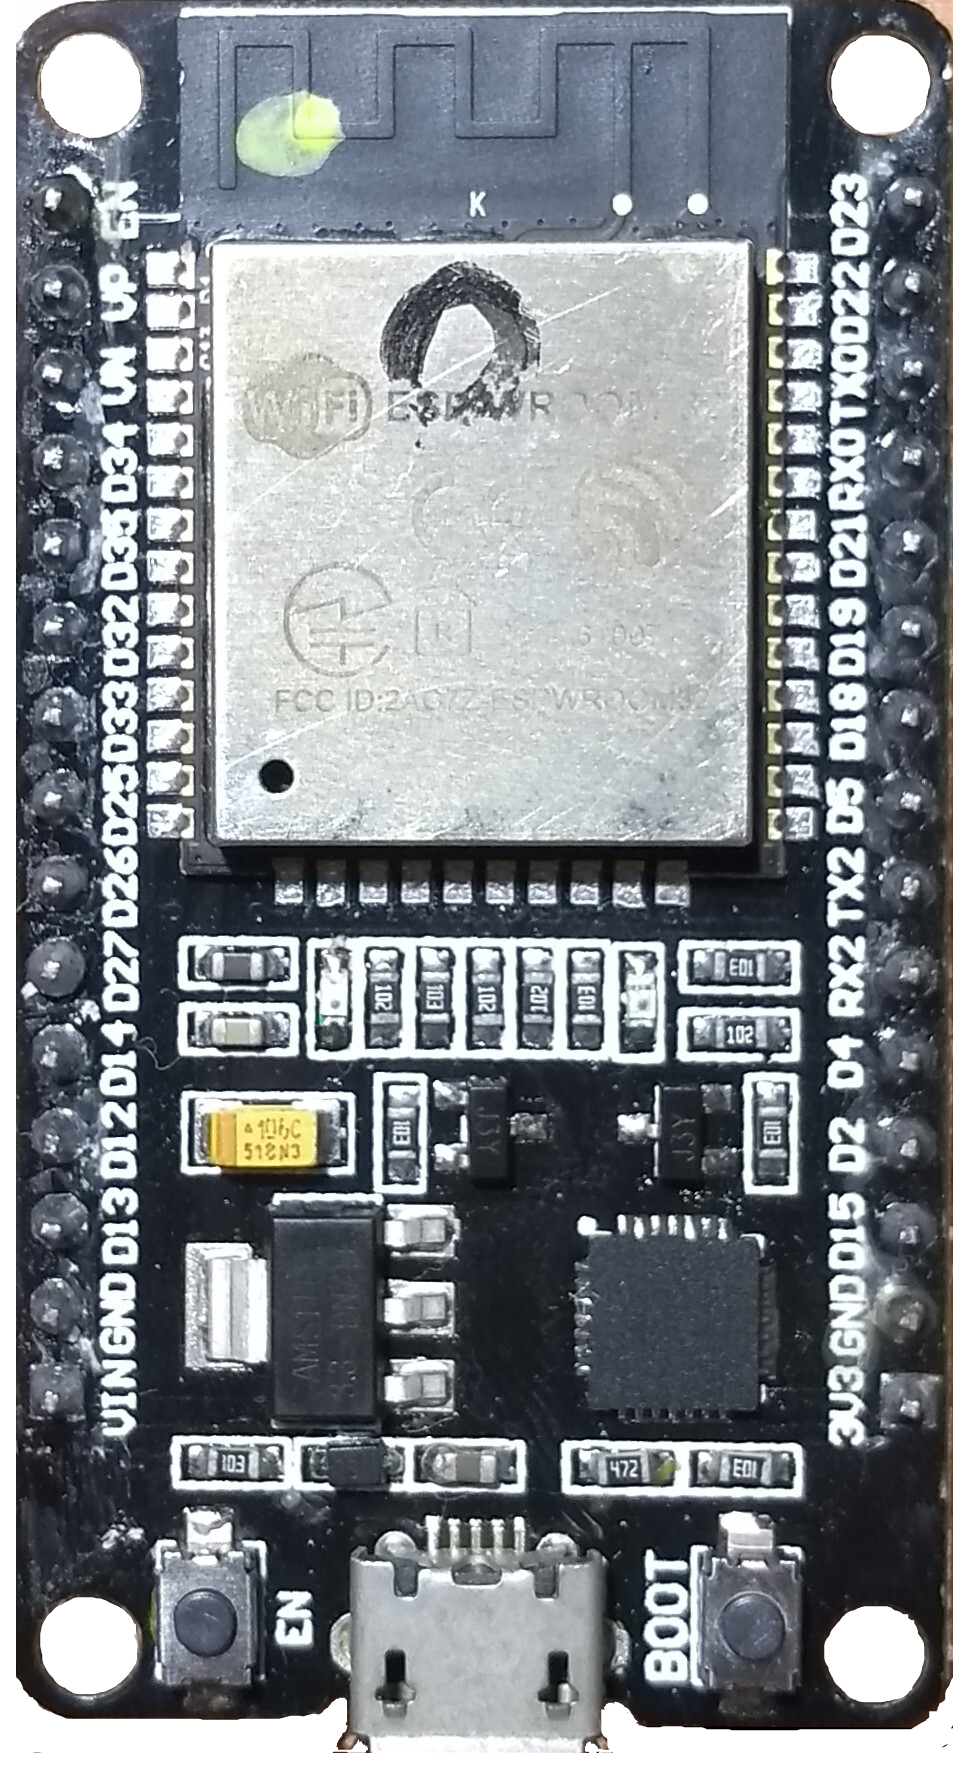
\includegraphics[width=3cm]{imagens/eletronica/esp32_kit.png}
    \caption{Placa de desenvolvimento ESP32 Dev1.}
    \label{fig:esp32_kit}
\end{figure}

\begin{figure}[H]
    \centering
    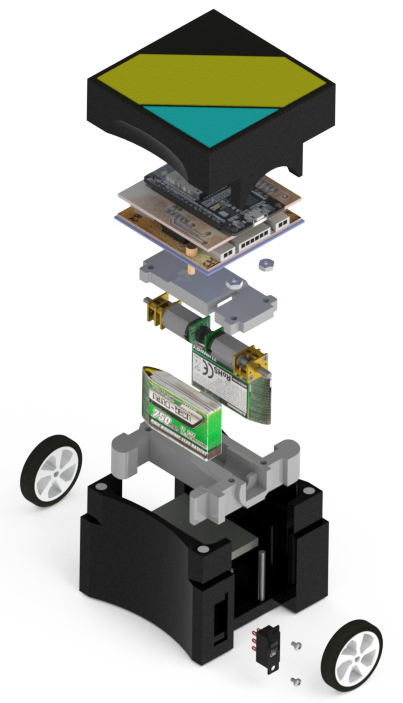
\includegraphics[width=5cm]{imagens/robo_completo_explodido.png}
    \caption{Vista explodida do robô completo.}
    \label{fig:robo_completo_explodido}
\end{figure}

\subsection{Placa de Circuito Impresso}
% CIRCUITO ELÉTRICO/ELETRÔNICO COMPLETO
% MOSTRAR/EXPLICAR: PLACA DE CIRCUITO IMPRESSO DESENVOLVIDA
% TODO:
% ref:  https://produza.ind.br/gestao/pre-requisitos-tecnicos-para-montar-um-projeto-eletronico/

% \begin{figure}[H]
%     \centering
%     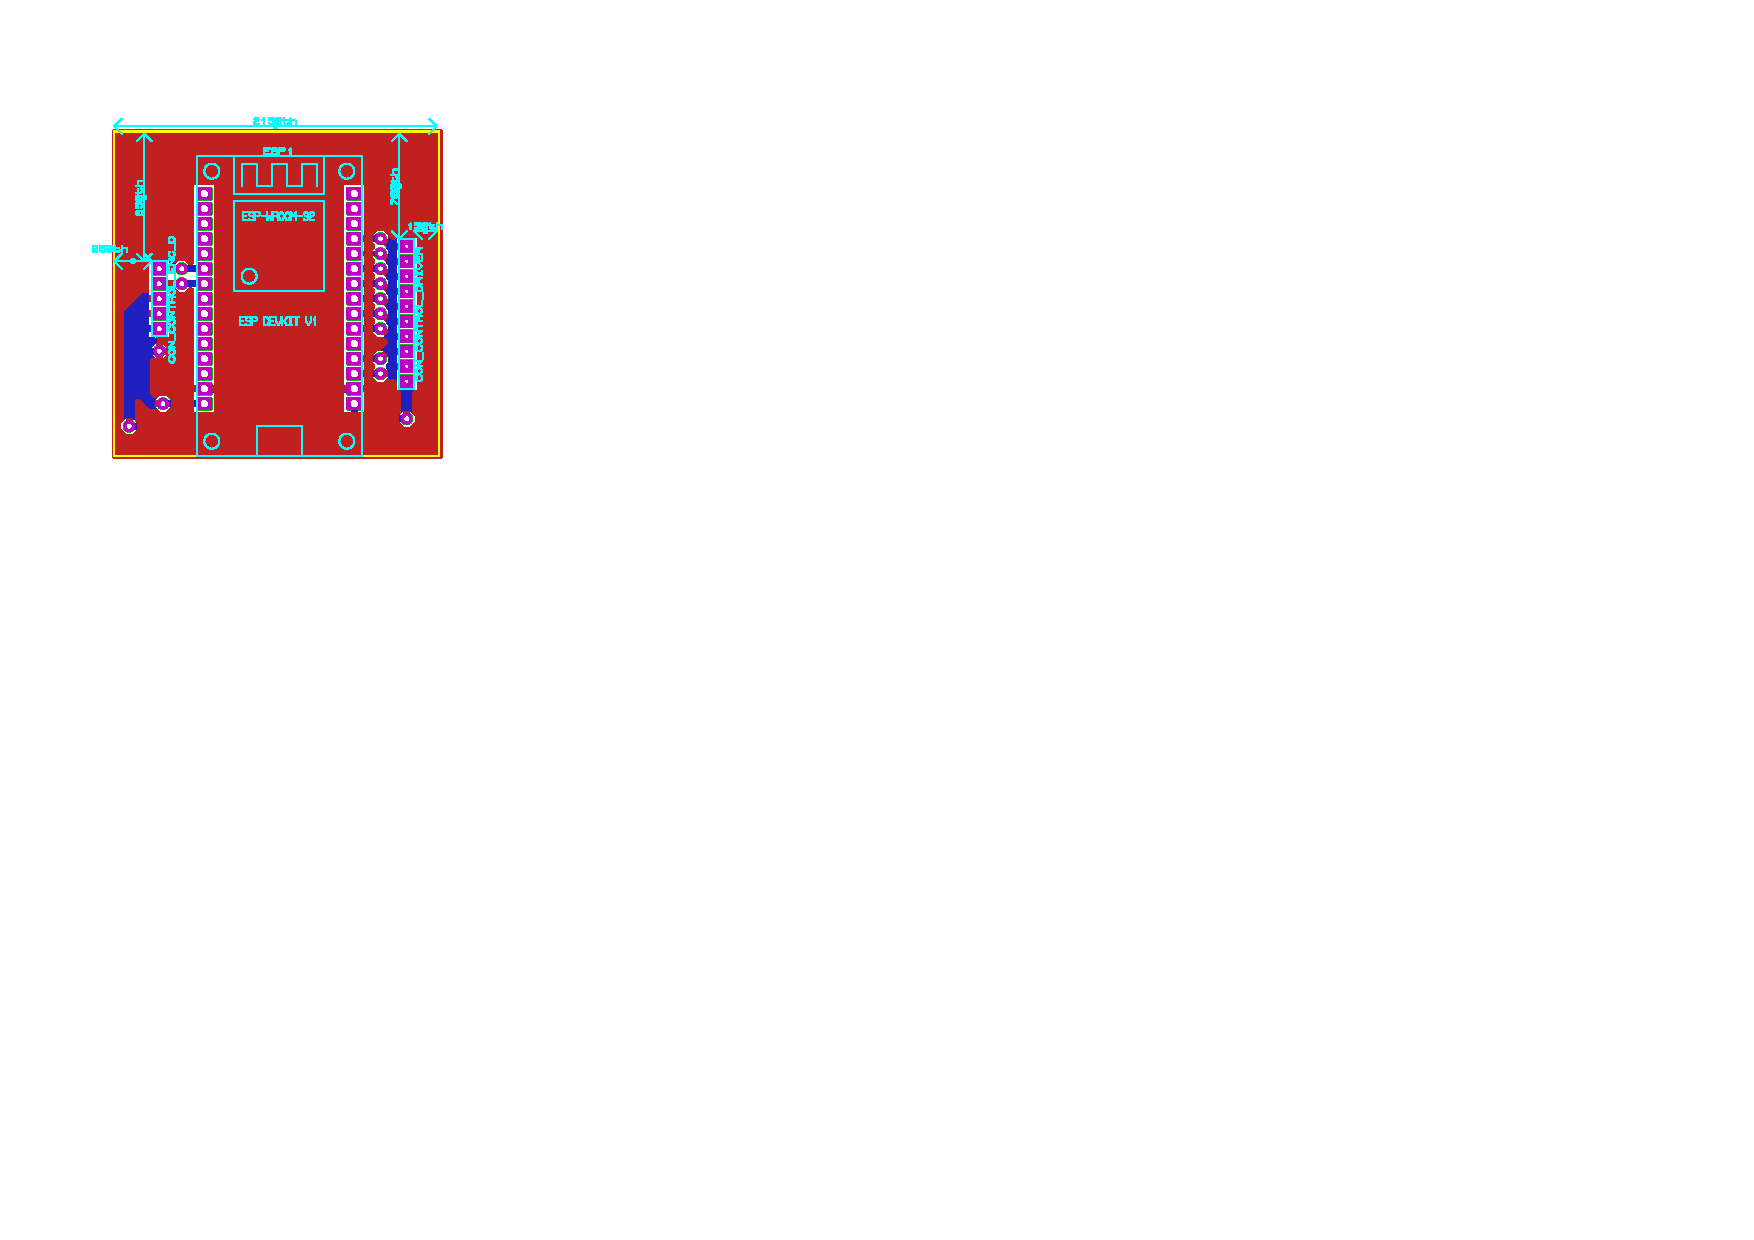
\includegraphics[width=\textwidth]{imagens/eletronica/placa/placa_controle_completa.pdf}
%     \caption{Caption}
%     % \label{fig:my_label}
% \end{figure}

% \begin{figure}[H]
%     \centering
%     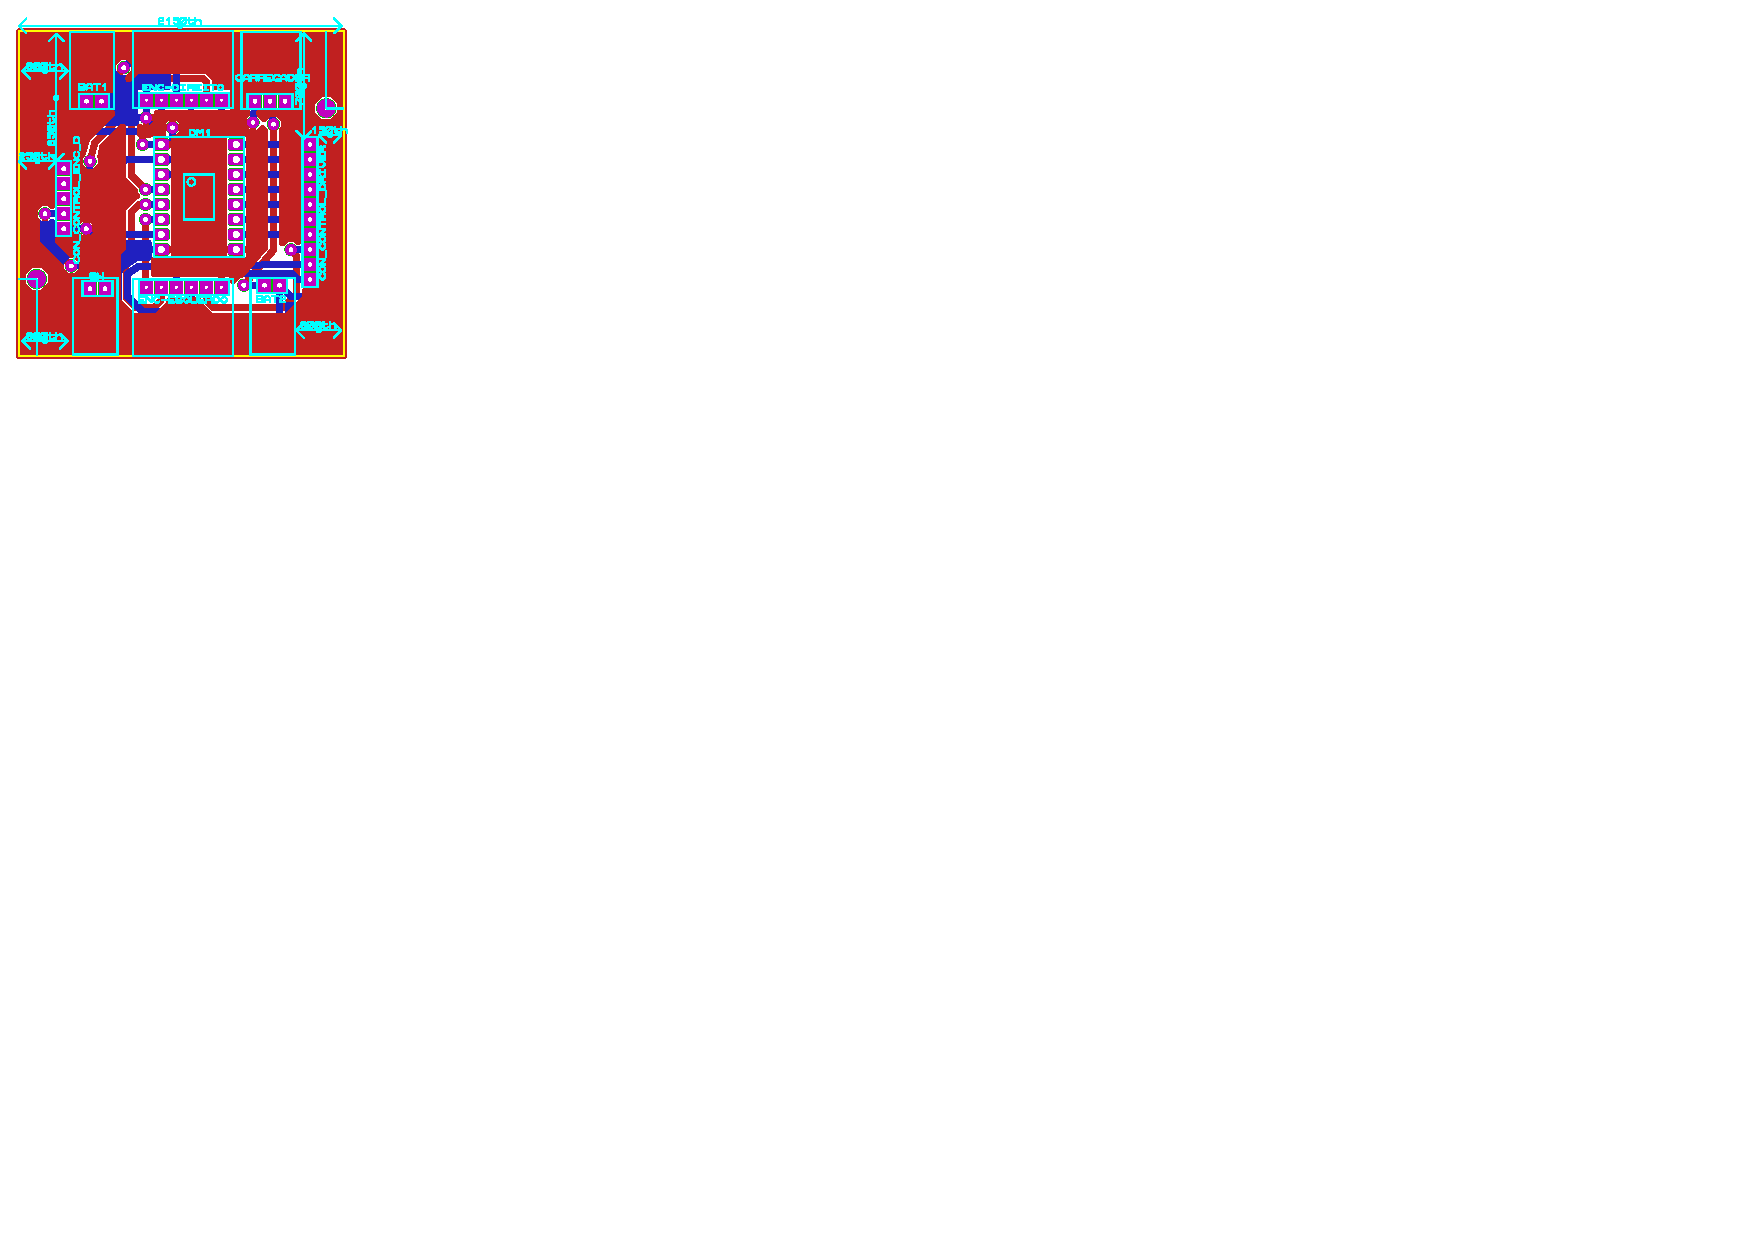
\includegraphics[width=\textwidth]{imagens/eletronica/placa/placa_driver_completa.pdf}
%     \caption{Caption}
%     % \label{fig:my_label}
% \end{figure}

\begin{enumerate}
    \item \textbf{Concepção inicial}:
        O principal objetivo por trás de se fazer uma nova placa de circuito eletrônico é acomodar os componentes, respeitando os limites das dimensões estabelecidos pela competição na qual os robôs serão utilizados (caber dentro de um cubo de $75$ mm de aresta). A placa deve conter o microcontrolador, no seu kit de desenvolvimento, \textit{Driver motor} para acionamento dos motores DCs, os \textit{Encoders} e ser alimentada por duas baterias de $1$ célula do tipo \textit{Lipo}.
        
    \item \textbf{Elaboração dos esquemáticos eletrônicos}:
        O esquemático foi a parte mais simples, pois não houve grandes mudanças nessa parte, com relação aos projetos de anos anteriores. A maior mudança foi o microcontrolador, que provocou dificuldades maiores na etapa seguinte, a elaboração do \textit{Layout}, devido às dimensões dos componentes.
        
        % inserir imagem do esquemático geral aqui
        
        \begin{figure}[H]
            \centering
            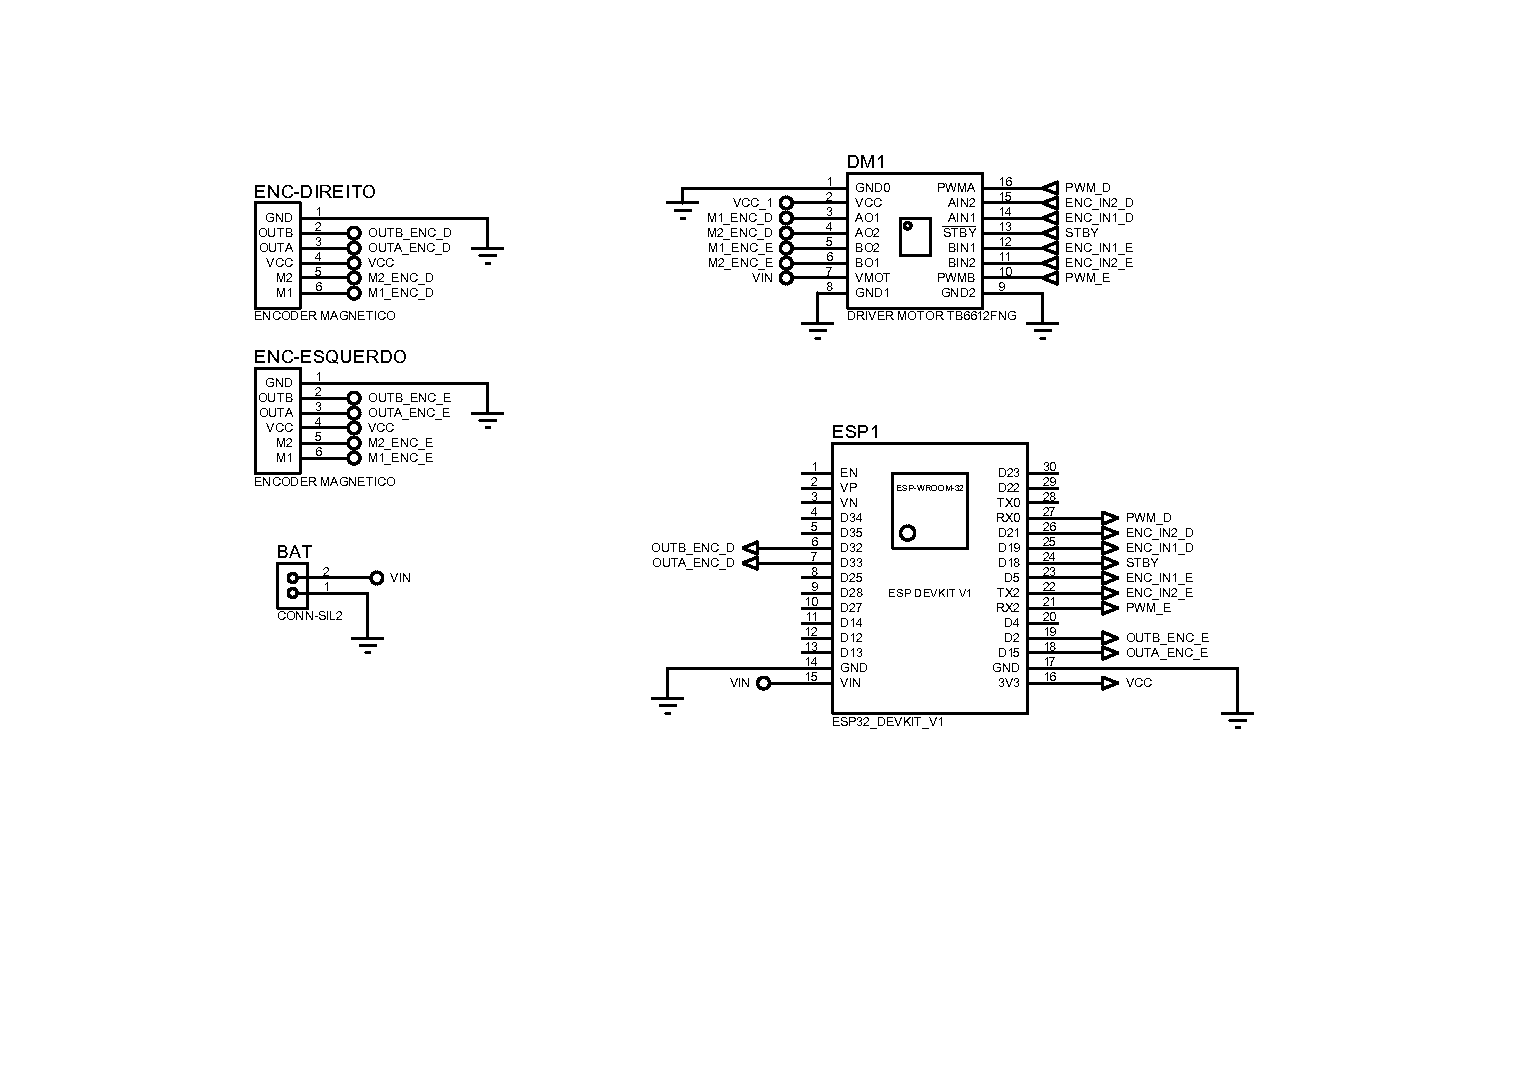
\includegraphics[width=\textwidth]{imagens/eletronica/placa/esquematico_completo.pdf}
            \caption{Esquemático.}
        \end{figure}
        
    \item \textbf{Elaboração do layout}:
        % inserir imagem do layout final aqui
        Este ponto foi o mais crítico nessa tarefa, devido à restrição de tamanho da placa ser de um quadrado com até $55$mm de lado. A solução adotada foi fazer em duas camadas, ou seja, duas placas cobreadas, ambas dupla face, dividindo os componentes. Em uma placa foi comportado o \textit{Driver}, bem como os conectores para os motores com os sensores e os conectores das baterias, e na outra apenas o microcontrolador. Para a conexão entre as placas foi utilizado um conector do tipo \textit{Head}, um macho e uma fêmea. Dessa forma, as placas conseguiram respeitar o limite dimensional e comportar todos os componentes necessários.
    \item \textbf{Realização de testes}:
        % faltou imagem de testes aqui
        Foram realizados testes antes da concepção da PCI, em \textit{Protoboards} para conferir se o circuito está funcionando como esperado e após a confecção, para se verificar a qualidade da confecção das placas.
        
        Também foram realizados testes individuais nos componentes, principalmente nos sensores, com o uso de osciloscópios. Verificou-se o funcionamento correto dos \textit{Encoders} e também conferiu-se se a distância entre os sensores poderia estar gerando interferência um no outro. Os resultados desses testes foram que todos os \textit{encoders} utilizados estão em bom estado, ou seja, funcionando como esperado e a distância que eles ficarão ao serem acomodados na estrutura não causa interferência um no outro.
    \item \textbf{Verificação e validação}
        Após testes individuais, de cada componente, foram realizados testes com a montagem completa, ou seja, os robôs montados por completo com as PCIs, baterias, motores e sensores. A validação foi por meio de controle manual dos robôs e testes simples de leitura de \textit{Encoder}, pois nessa etapa o \textit{Firmware} ainda não havida sido implementado.
\end{enumerate}

\subsection{O \emph{Firmware}}
% Falar sobre como foi feito a divisão das atividades no microcontrolador
% Mostrar ilustração dessa divisão, para ter-se uma visão global das rotinas e suas relações de dependência

\subsubsection{Rotina de Calibração}

Rotina responsável por realizar a identificação dos parâmetros do modelo dos motores direito e esquerdo do robô: constante de tempo; ganho de malha aberta; parâmetros do controlador \emph{FeedForward}; velocidade máxima de cada motor. Bem como calcular os ganhos para o controlador \emph{PID} de forma a se obter uma resposta pré-definida em malha fechada.\\

A rotina de calibração consiste em três etapas que são repetidas para todas as configurações: motor direito para frente; motor direito para trás; motor esquerdo para frente e motor esquerdo para trás. Cada etapa é descrita a seguir: 

% TO DO:
% ORGANIZAR E REPENSAR A FORMA DE EXIBIR AS ETAPAS
% FIGURAS ILUSTRANDO O COMPORTAMENTO GERAL DAS FUNÇÕES QUE ESTÃO SENDO USADAS NA INTERPOLAÇÃO
% PSEUDO CÓDIGOS TALVEZ
\begin{itemize}
    \item \textbf{ETAPA 1}: Estimar a zona morta e o ganho da planta em malha aberta\\
    
    Para isso é realizado a coleta de $N$ pontos ($\omega$,$u$), o primeiro ponto é coletado para $u = \pm1$(valor máximo no sentido de giro atual) e é realizado sucessivos decréscimos neste valor até a parada do motor ($\omega = 0$). \\
    
    Aplicar sinal de controle atual ($u_i$);\\
    Aguardar um tempo fixo, pré-determinado, para garantir a leitura de $\omega_{ss}$(velocidade de máxima/velocidade de regime)
    Armazenar ($u_i$,$\omega_{ss}$).\\
    
    A aquisição destes pontos ocorre da maior velocidade para a menor devido à zona morta ser mais baixa neste sentido, por causa da inercia do motor.\\
    
    Ao se encerrar a coleta destes pontos ($\omega_{ss} = 0$ detectado) é realizado uma regressão linear por \textit{MMQ}, tendo $\omega$ no eixo das ordenadas e $u$ no eixo das abscisas, o coeficiente angular dessa reta relaciona a velocidade angular ($\omega$) com o sinal de controle ($u$), já o coeficiente linear representa a zona morta, ou seja, o menor $u$ que pode iniciar o giro do motor.
    
    \begin{equation*}
        u(\omega) = a\omega + b
    \end{equation*}
    
    Com esses parâmetros dessa reta é possível estimar o ganho de malha aberta da planta da seguinte forma:
    
    \begin{equation*}
        K = \frac{(u_{max} - b)}{a}
    \end{equation*}
        
    \begin{figure}[H]
        \centering
        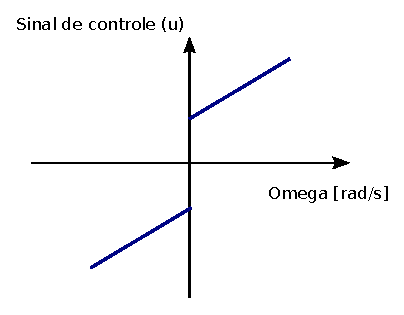
\includegraphics[width=0.5\textwidth]{imagens/ilustracoes/omega_x_sinal_controle.eps}
        \caption{Comportamento da curva $u(\omega)$.}
        \label{fig:ilustracao_omega_x_pwm}
    \end{figure}    
        
    \item \textbf{ETAPA 2}: Estimar a constante de tempo
    
    Para obter a constante de tempo da planta na configuração atual, faz-se uso mais uma vez de interpolação por \textit{MMQ} e tira-se proveito do conhecimento do ganho da planta para simplificar e tornar possível essa interpolação de forma simples. Para estimar a constante de tempo obtém-se $M$ pontos ($t$,$\omega$) e aplica-se o \textit{MMQ} para uma interpolação linear, para isso é necessário fazer a seguinte alteração:
        

    \begin{align*}
        \omega(t) &= K\left( 1 - e^{-t/T_m} \right)\\
        \ln{\omega(t)} &= \ln\left[K( 1 - e^{-t/T_m})\right]\\
        \ln\left(1 - \frac{\omega(t)}{K} \right) &= -\frac{t}{T_m}\\
        y_{aux}(t) &= -\frac{t}{T_m}
    \end{align*}
    
    Convertendo $\omega(t)$ para $y_{aux}(t)$ o coeficiente angular resultante da interpolação linear será: $coef.angular = -\frac{1}{T_m}$, dessa forma obtemos a constante de tempo.
    
    \item \textbf{ETAPA 3}: Calcular os parâmetros do controlador \textit{PID}
    
    Como apresentado na seção de referencial teórico é possível relacionar o ganho do controlador proporcional com o polo desejado para o sistema em malha fechada, por meio da relação (??). Esse cálculo só é possível devido a identificação dos parâmetros da planta resultante das etapas anteriores. O polo desejado para todas as configurações da planta é uma constante pré-definida pelo usuário.
    
\end{itemize}

Ao se passar por todas as configurações de motor/sentido a rotina seleciona a menor velocidade máxima apresentada por alguma dessas configurações e armazena esta velocidade como sendo a velocidade máxima atingida pelos motores deste robô, isso é importante, para assegurar que a referencia $\omega_{ref}$ seja factível para todas as configurações. \\

Por fim os resultados são armazenados na memória permanente do microcontrolador, sendo atualizado/sobrescrita apenas ao final da próxima chamada da rotina de calibração.

\subsubsection{Rotina de Comunicação}
% TODO:
% IDEIA: ILUSTRAR A INTERAÇÃO ENTRE A ROTINA PRINCIPAL E A INTERRUPÇÃO
A rotina de comunicação opera em um \emph{loop} infinito no núcleo principal do microcontrolador e é responsável por tratar os telecomandos recebidos pelo \textit{Bluetooth}. Ao ser identificado um recebimento de mensagem pela sinal de interrupção da comunicação \textit{Bluetooth} é acionado a função de tratamento de interrupção correspondente que possui como única função encaminhar as mensagens válida (verificar cabeçalho) para a rotina principal de comunicação. Isso é feito para evitar sobrecarregar a interrupção, já que ela deve operar em altas frequências.\\

Na rotina principal a mensagem é interpretada e caso ela seja identificado um telecomando válido, será executado a devida resposta, conforme apresentado a seguir.

O protocolo implementado, foi pensado para conter até três grandes campos, o \textbf{\textit{Head}} com 4 bits de preambulo, para ajudar a sincronizar os pacotes, o \textbf{\textit{Cmd}} também com 4 bits, possibilitando assim até 16 comandos distintos e o campos de argumentos com tamanho variável. Foram implementados 7 comandos. 

% Please add the following required packages to your document preamble:
% \usepackage[table,xcdraw]{xcolor}
% If you use beamer only pass "xcolor=table" option, i.e. \documentclass[xcolor=table]{beamer}
\begin{table}[H]
\centering
\begin{tabular}{c|r}
\hline
\rowcolor[HTML]{C0C0C0} 
\multicolumn{1}{|c|}{\cellcolor[HTML]{C0C0C0}DEFINIÇÕES} & \multicolumn{1}{r|}{\cellcolor[HTML]{C0C0C0}VALOR(HEX)} \\ \hline
HEAD & A0 \\
\rowcolor[HTML]{EFEFEF} 
CMD\_REQ\_CAL & 00 \\
CMD\_REQ\_OMEGA & 03 \\
\rowcolor[HTML]{EFEFEF} 
CMD\_CALIBRATION & 04 \\
CMD\_IDENTIFY & 05 \\
\rowcolor[HTML]{EFEFEF} 
CMD\_SET\_POINT & 0A \\
CMD\_CONTROL\_SIGNAL & 0B \\
\rowcolor[HTML]{EFEFEF} 
CMD\_PING & 0F
\end{tabular}
\caption{Definições utilizadas.}
\label{tab:my-table}
\end{table}
    
\textbf{Comandos}
\begin{itemize}
    \item \textbf{CMD\_REQ\_CAL}:\\
        \textit{Host} envia, para solicitar os dados provenientes da calibração do controlador \textit{feedforward}. O escravo (robô) envia 4 \emph{floats}, referente aos coeficientes do controlador.
    \item \textbf{CMD\_REQ\_OMEGA}:\\
        \textit{Host} envia, para solicitar as velocidades atuais de ambos os motores, em $rad/s$. O escravo responde com dois \emph{floats}, referentes aos ômegas em cada motor.
    \item \textbf{CMD\_CALIBRATION}:\\
        \textit{Host} envia, para fazer com que o robô inicie sua rotina de calibração do controlador.
    \item \textbf{CMD\_IDENTIFY}:\\
        \textit{Host} envia, fazendo com que o robô inicia sua rotina de identificação. O \textit{Host} deve enviar o \emph{bitstream} da seguinte forma:\\
        
        % Please add the following required packages to your document preamble:
% \usepackage{graphicx}
% \usepackage[table,xcdraw]{xcolor}
% If you use beamer only pass "xcolor=table" option, i.e. \documentclass[xcolor=table]{beamer}
\begin{table}[H]
\centering
\resizebox{\textwidth}{!}{%
\begin{tabular}{|
>{\columncolor[HTML]{C0C0C0}}l |
>{\columncolor[HTML]{C0C0C0}}l |l|l|l|}
\hline
HEAD & CMD\_IDENTIFY & OPTIONS & SETPOINT & STEPTIME \\ \hline
\end{tabular}%
}
\end{table}
        
        Sendo o campos \textbf{options} de 1 byte, contendo a informação de qual motor será feita a identificação e se deve ser usado o controlador.
        
        Ao concluir a rotina de identificação, o robô responde enviando o vetor de ômegas medidos, durante a rotina, para o \textit{host}, que deve estar aguardando recebê-las. A quantidade de dados será $\frac{timeout}{steptime}*4$ bytes, portando o \textit{host} deve estar aguardando exatamente essa quantidade de bytes.
        
        
    \item \textbf{CMD\_SET\_POINT}:\\
        
        % Please add the following required packages to your document preamble:
% \usepackage{graphicx}
% \usepackage[table,xcdraw]{xcolor}
% If you use beamer only pass "xcolor=table" option, i.e. \documentclass[xcolor=table]{beamer}
\begin{table}[H]
\centering
\resizebox{\textwidth}{!}{%
\begin{tabular}{|
>{\columncolor[HTML]{C0C0C0}}c |
>{\columncolor[HTML]{C0C0C0}}c |c|c|c|c|l|l|l|}
\hline
HEAD & CMD\_SET\_POINT & SENSE\_L & OMEGA\_L & SENSE\_R & \multicolumn{4}{c|}{OMEGA\_R} \\ \hline
\end{tabular}%
}

\end{table}
        
        Neste os campos de \textbf{sense\_x} indicam o sentido de rotação do motor, 0 para trás e 1 para rodar para frente (convertidos em sinal dos ômegas de setpoint), portando só ocupam 1 bit, já os campos referentes aos ômegas desejados ocupam 15 bits, sendo assim é possível enviar referências com uma precisão de $1.0/2^{15}$, já que as referências serão enviadas inteiras  (0 - $2^{15}$) e mapeadas de $-1.0$ a $1.0$, indicando uma porcentagem da referência da velocidade máxima do robô. Ou seja os campos referentes aos \textit{setpoints} contêm a porcentagem da velocidade máxima do robô.
        
    \item \textbf{CMD\_CONTROL\_SIGNAL}:\\
        
        O comando difere apenas o campo de \textbf{cmd} do comando anterior. O restante da estrutura é exatamente igual, pois a principal diferença ocorre no microcontrolador. Em vez dos campos referentes aos ômegas serem porcentagens da velocidade máxima que será convertido em \textit{Setpoint} para o controlador, neste comando o robô irá interpretar esses campos como sendo sinais de controle (após convertê-los para \emph{float} de $-1.0$ a $1.0$).
        
    \item \textbf{CMD\_PING}:\\
        Neste comando o \textit{host} pode enviar qualquer mensagem no campo de argumentos, pois o robô irá apenas responder com a mesma mensagem. Este comando é útil para testar conexão e testar a latência da conexão.
    
\end{itemize}

% TABELA TEMPORÁRIA
\begin{table}[H]
\resizebox{\textwidth}{!}{
\begin{tabular}{|l|c|c|l|}
\hline
\multicolumn{1}{|c|}{Command Tag} & \multicolumn{1}{l|}{Hex} & Arg. & \multicolumn{1}{c|}{Description} \\ \hline
CMD\_REQ\_CAL & 0x00 & - & \begin{tabular}[c]{@{}l@{}}Solicita ao microcontrolador que envie os\\ dados da última calibração, que estão armazenados na memória flash.\end{tabular} \\ \hline
 &  &  &  \\ \hline
 &  &  &  \\ \hline
CMD\_REQ\_OMEGA & 0x03 & - & \begin{tabular}[c]{@{}l@{}}Solicita ao microcontrolador que envie as leituras atuais da velocidade\\ de rotação, em rad/s, dos dois motores. O microcontrolador enviará dois\\ floats, sendo primeiro float refererente ao motor esquerdo e o segundo ao\\ motor direito.\end{tabular} \\ \hline
CMD\_CALIBRATION & 0x04 & - & \begin{tabular}[c]{@{}l@{}}Sinaliza para o microcontrolador que ele deve iniciar a rotina de calibração\\ dos parâmetros do controlador, bem como os parâmetros para o filtro de Kalman.\end{tabular} \\ \hline
CMD\_IDENTIFY & 0x05 & - & \begin{tabular}[c]{@{}l@{}}Sinaliza para o microcontrolador que ele deve iniciar a rotina \\ de coleta dos dados  de identificação e ao final deve enviar \\ esses dados para o host.\end{tabular} \\ \hline
 &  &  &  \\ \hline
 &  &  &  \\ \hline
 &  &  &  \\ \hline
 &  &  &  \\ \hline
CMD\_REF & 0x0A & \begin{tabular}[c]{@{}c@{}}ref. Left (15bits)\\ ref.Right (15 bits)\end{tabular} & \begin{tabular}[c]{@{}l@{}}Informa ao microcontrolador qual referência aplicar para \\ o controlador de velocidade de rotação. \\ As referências estão no intervalo {[}-1.0, 1.0{]}.\end{tabular} \\ \hline
CMD\_CONTROL\_SIGNAL & 0x0B & \begin{tabular}[c]{@{}c@{}}pwm. Left (15bits)\\ pwm.Right (15 bits)\end{tabular} & \begin{tabular}[c]{@{}l@{}}Informa ao microcontrolador qual sinal de controle aplicar. \\ Valores no intervalo {[}-1.0, 1.0{]}.\end{tabular} \\ \hline
 &  &  &  \\ \hline
 &  &  &  \\ \hline
CMD\_RESET & 0x0E &  &  \\ \hline
CMD\_PING & 0x0F & mensagem qualquer & Sinaliza para o microcontrolador que ele deve apenas devolver a mensagem para o host. \\ \hline
\end{tabular}
}
\caption{}
\label{tab:command_table}
\end{table}

\subsubsection{Rotina de Controle}
% TODO:
O controle é executado sozinho no núcleo secundário do ESP32 em \emph{loop} infinito com uma taxa de atualização de $5ms$. A rotina consiste em receber as velocidades providas pela de leitura dos sensores por meio de mensagens entre processos, em seguida é realizado a etapa de controle propriamente dita, que consiste em aplicar a ação do controle \textit{FeedForward} somado a ação do controle de malha fechada, tendo como entrada a última referência de percentual de velocidade lida pela rotina de comunicação multiplicada pela velocidade máxima considerada para a rotação do eixo do motor, para passar a referência para $rad/s$. \\

Ao final do fluxo de controle tem-se o sinal de controle, este por sua vez é utilizado para configurar o sentido de giro e o sinal \emph{PWM} que deve ser aplicado no \emph{Driver} motor correspondente.

\subsubsection{Rotina de Leitura dos Sensores}
% TODO:
% REALIZAR ANÁLISE DE FREQ. MÁXIMA DE OPERAÇÃO DOS ENCODERS VS BANDA DISPONIVEL NAS INTERRUPÇÕES RESPONSAVEIS PELA LEITURA DOS ENCODERS

Há duas interrupções associadas aos sinais provenientes dos \emph{Encoders} rotativos, uma para cada motor, cujo objetivo é calcular/medir a velocidade de rotação do eixo do motor ($\omega_{medido}$) bem como aplicar o filtro de \emph{Kalman} para uma melhor estimativa da mesma. As interrupções são provocadas pelas bordas dos pulsos de ambos os canais, fazendo com que a resolução do sensor seja utilizada ao máximo, pois dessa maneira os sensores que possuem uma resolução de três pulsos completos por revolução (em cada canal, ver Figura \ref{fig:ilustracao_uma_revolucao}) consegue acionar doze ($12$) vezes a interrupção que irá computar o $\omega_{motor}$, passando assim a ser ter uma resolução de doze pulsos por revolução.\\

Para o cálculo do módulo da velocidade de rotação do eixo do motor faz-se:
\begin{equation}
    |\omega_{medido}| = \frac{2\pi}{NPR}\frac{1}{\Delta{t}}
    \label{eq:modulo_omega_medido}
\end{equation}

Onde $NPR$ é o número pulsos por revolução em um canal. Neste trabalho o $NPR$ é igual a três($3$). Já o intervalo $\Delta{t}$ é o intervalo entre bordas iguais em um canal, a Figura \ref{fig:sinal_em_quadratura_delta_t} ilustra esse intervalo para as bordas de subida de ambos os canais.\\

\begin{figure}[H]
    \centering
    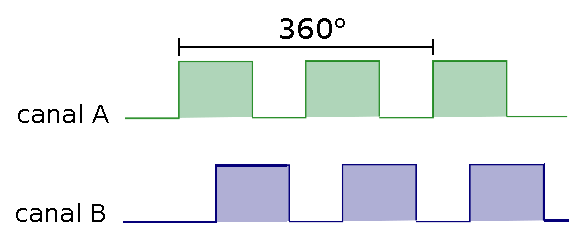
\includegraphics[width=0.5\textwidth]{imagens/ilustracoes/sinal_enquadratura_uma_revolucao.eps}
    \caption{Ilustração do sinal em quadratura em uma revolução completa do eixo do motor no sentido horário.}
    \label{fig:ilustracao_uma_revolucao}
\end{figure}

\begin{figure}[H]
    \centering
    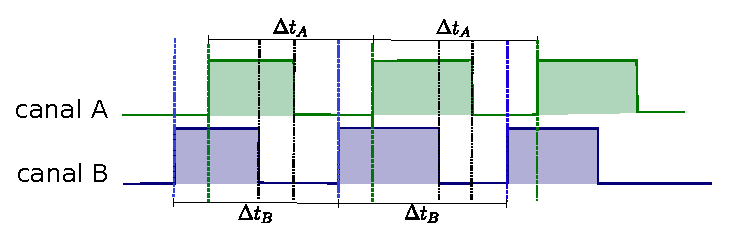
\includegraphics[width=0.6\textwidth]{imagens/ilustracoes/sinal_em_quadratura_sentido_CCW_detalhada.eps}
    \caption{Ilustração de um sinal em quadratura para uma revolução do eixo do motor sentido anti-horário para um \emph{Encoder} com a resolução de três pulsos por revolução, com destaque para o intervalo de tempo entre as bordas de subida de um mesmo canal.}
    \label{fig:sinal_em_quadratura_delta_t}
\end{figure}

% Please add the following required packages to your document preamble:
% \usepackage{graphicx}
\begin{table}[H]
\centering
\resizebox{0.5\textwidth}{!}{%
\begin{tabular}{cc|cc}
\multicolumn{2}{c|}{\textbf{\begin{tabular}[c]{@{}c@{}}Sentido\\     Horário\end{tabular}}} &
  \multicolumn{2}{c}{\textbf{\begin{tabular}[c]{@{}c@{}}Sentido\\ Anti-Horário\end{tabular}}} \\ \hline
\textbf{A} & \textbf{B} & \textbf{A} & \textbf{B} \\
1          & 0          & 1          & 0          \\
0          & 1          & 0          & 1         
\end{tabular}%
}
\caption{Código de 2 bits para identificar o sentido de rotação.}
\label{tab:tabela_simple_code}
\end{table}

Já para se obter o sentido de rotação do motor, faz-se uso do padrão \emph{Gray Code} gerado pela diferença de fase entre os diferentes canais de um mesmo sensor, uma maneira de fazer isso é ler os \emph{GPIO}'s associados aos canais do \emph{Encoder} e verificar o padrão em binário e inferir o sentido de rotação, a Figura \ref{fig:cw_signal} ilustrado isso para uma rotação no sentido horário e a Figura \ref{fig:ccw_signal} o anti-horário, esses códigos são apresentados na Tabela \ref{tab:tabela_simple_code}. Porém esse procedimento apresentou ser pouco eficiente em medias e altas rotações, devido a alta taxa de erro na inferência do sentido. \\


A abordagem adotada aqui foi armazenar os dois \emph{bits}(sendo canal A bit mais significado) e concatenar/somar com os últimos dois \emph{bits} (da leitura anterior) deslocados em dois (equivalente à multiplicar por $2^2$ ou operar bit-a-bit: $bits_{anteriores} \ll 2$), criando assim um padrão com $4$ \emph{bits}, sendo os dois mais significados o padrão da leitura anterior e os dois menos significativos a leitura atual. Esse procedimento é ilustrado para uma rotação no sentido horário e no sentido anti-horário respectivamente nas Tabelas \ref{tab:tabela_gray_code_cw} e \ref{tab:tabela_gray_code_ccw}, dessa forma gera-se quatro($4$) padrões/códigos que caracterizam um tipo de rotação. Esse padrão de $4$\emph{bits} é armazenado de forma estática em um vetor(uma tabela de cola/ \emph{lookup table}) nas rotinas de ambos os motores, esse vetor mapeia o código binário em $1$, $-1$ ou zero para as combinações que não caracterizam um sentido de giro, o sinal do valor corresponde ao sentido horário ou anti-horário e depende do motor, um exemplo de \emph{lookup table} é apresentado na Tabela \ref{tab:lookup_table}.

\begin{figure}[H]
    \centering
    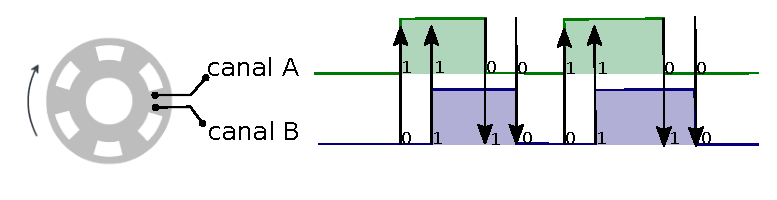
\includegraphics[width=0.7\textwidth]{imagens/ilustracoes/sinal_enquadratura_sentido_CW.eps}
    \caption{Sinal em quadratura para rotação no sentido horário.}
    \label{fig:cw_signal}
\end{figure}

% Please add the following required packages to your document preamble:
% \usepackage{graphicx}
\begin{table}[H]
\centering
\resizebox{0.5\textwidth}{!}{%
\begin{tabular}{c|c|c|c|c}
\textbf{$A_{ant}$} & \textbf{$B_{ant}$} & \textbf{$A_{atual}$} & \textbf{$B_{atual}$} & \textbf{DEC} \\ \hline
0 & 0 & 1 & 0 & 2 \\
1 & 0 & 1 & 1 & 11 \\
1 & 1 & 0 & 1 & 13 \\
0 & 1 & 0 & 0 & 4
\end{tabular}%
}
\caption{Gray Code para a rotação no sentido horário.}
\label{tab:tabela_gray_code_cw}
\end{table}

\begin{figure}[H]
    \centering
    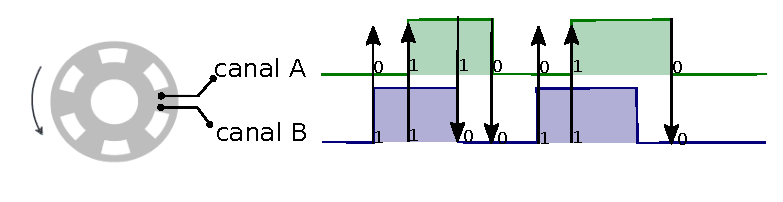
\includegraphics[width=0.7\textwidth]{imagens/ilustracoes/sinal_enquadratura_sentido_CCW.eps}
    \caption{Sinal em quadratura para rotação no sentido anti-horário.}
    \label{fig:ccw_signal}
\end{figure}

% Please add the following required packages to your document preamble:
% \usepackage{graphicx}
\begin{table}[H]
\centering
\resizebox{0.5\textwidth}{!}{%
\begin{tabular}{c|c|c|c|c}
\textbf{$A_{ant}$} & \textbf{$B_{ant}$} & \textbf{$A_{atual}$} & \textbf{$B_{atual}$} & \textbf{DEC} \\ \hline
0 & 0 & 0 & 1 & 1  \\
0 & 1 & 1 & 1 & 7  \\
1 & 1 & 1 & 0 & 14 \\
1 & 0 & 0 & 0 & 8 
\end{tabular}%
}
\caption{Codificação de 4 \emph{bits} para a rotação no sentido anti-horário.}
\label{tab:tabela_gray_code_ccw}
\end{table}

% Please add the following required packages to your document preamble:
% \usepackage{graphicx}
\begin{table}[H]
\centering
\resizebox{0.8\textwidth}{!}{%
\begin{tabular}{c|ccccllllllllllll}
\textbf{Índice} & 0 & 1  & 2 & 3 & 4 & 5 & 6 & 7  & 8  & 9 & 10 & 11 & 12 & 13 & 14 & 15 \\ \hline
\textbf{Valor}  & 0 & -1 & 1 & 0 & 1 & 0 & 0 & -1 & -1 & 0 & 0  & 1  & 0  & 1  & -1 & 0 
\end{tabular}%
}
\caption{Lookup table.}
\label{tab:lookup_table}
\end{table}

Com a \emph{lookup table} e o módulo da velocidade é possível calcular a velocidade de rotação da seguinte forma:

\begin{equation}
    \omega_{medido} = \frac{2\pi}{NPR}\frac{table[code]}{\Delta{t}}
\end{equation}

A próxima etapa é a filtragem dessa velocidade, a rotina aplica o filtro de \emph{Kalman} (mais detalhes na seção de referencial teórico) considerando $omega(t)$ um sistema de primeira ordem, como apresentado na seção sobre modelagem de motores de corrente contínua essa pode ser uma boa aproximação se desconsiderar a influência da indutância interna do motor, isso faz com as variáveis do filtro sejam modeladas para:


\begin{equation*}
\begin{cases}
    \textbf{x}_k = \left[ \omega_k \right]\\
    z_k = x_k = \omega_k\\
    F_k = 1\\
    H_k = 1
\end{cases}
\end{equation*}

Modelo da \textbf{medição}:
\begin{align*}
z_k = \omega_{medido}
\end{align*}

Com isso a etapa de \textbf{predição} do filtro torna-se:
% MUDAR O SIMBOLO QUE FAZ REFERENCIA À ENTRADA (u) DE ENTRADA
\begin{align*}
    \check{\omega}_k &= \hat{\omega}_{k-1} + u_k\left( 1 - e^{-\Delta{t}/T_m} \right)\\
    \check{P}_k &= \hat{P}_{k-1} + Q_k
\end{align*}

Sendo $u_k$ a entrada no instante $k$, $\Delta t = t_f - t_0$. $\Delta t$ é relativo ao sinal de entrada $u_k$, sendo $t_0$ o instante que o sinal é aplicado e $t_f$ o instante atual $k$.


E a etapa de atualização \textbf{Atualização} é:

\begin{align*}
K_k &= \check{P}_k \left( \check{P}_k + R_k \right)^{-1} = \frac{\check{P}_k}{\check{P}_k + R_k}\\
\hat{\omega}_k &= \check{\omega}_k + K_k \left( \omega_{k_{medido}} - \check{\omega}_k \right)\\
\hat{P}_k &= \left( 1 - K_k \right) \check{P}_k
\end{align*}


% colocar aqui pseudo código da rotina completa

% \begin{algorithm}
% \caption{A Hough Transform for Squares Detection}
% \label{alg:hough_for_squares}
% \begin{algorithmic}[1]
% \State initialize $M$ with zero. \Comment{Voting matrix initialized with zero.}
% \ForAll{$(x',y')$ in $f(x,y)$}
%     \If{$|\nabla{f(x',y')}| \geq $ edge threshold } \Comment{It's an edge.}
        
%         \State $p_0 \gets (x',y')$
%         \State $\theta \gets \angle{\nabla{f(x',y')}} \mod{90^\circ}$ \Comment{Square's angle.}
%         \State $\Vec{N_0} \gets \nabla{f(x',y')}/|\nabla{f(x',y')}|$
%         \State $\Vec{N_1} \gets -\nabla{f(x',y')}/|\nabla{f(x',y')}|$
%         \State $\Vec{N_2} \gets$ rotate $\Vec{N_1}$ on $90^\circ$\\
        
        
%         \State Search for an edge point going in the direction of $\Vec{N_1}$ from $p_0$. \Comment{That will be the $p_1$ point.}\\
        
%         \State $l \gets |p_0 - p_1|$ \Comment{Square's size.}
        
%         \State $p_{middle} \gets (p_1 + p_0)/2$\\
        
%         \State Search for an edge point going in the direction of $\Vec{N_2}$ from $p_{middle}$. \Comment{That will be the $p_2$ point.}\\
        
%         \State $p_{center} \gets p_2 - \Vec{N_2}*l/2$ \Comment{$p_{center} = (x_c,y_c)$}
        
%         \State $M[x_c][y_c][l][\theta] \gets M[x_c][y_c][l][\theta] + 1$
        
%     \EndIf
% \EndFor
% \end{algorithmic}
% \end{algorithm}


% \subsubsection{Rotina de Telemetria}
% TODO:
% NOTA:
% Não sei se seria interessante falar dessa. Ao ser ativada ela inicia o armazenamento de vários dados, como velocidades, setpoint, velocidade filtrada, velocidade não filtrada, variáveis do filtro... grava esses dados durante x segundos e ao final envia tudo ao host via bluetooth
\section{RESULTADOS}
% APENAS PARA ILUSTRAR O TIPO DE PLOTS QUE PRETENDO COLOCAR
% CONSIGO REFAZER QUALQUER PLOT FACILMENTE
% TENHO INFORMAÇÃO/DADOS PARA GERAR DIVERSOS PLOTS E TESTES OFFLINE

% OBJETIVO:
% 1) MOSTRAR O RESULTADO DA CALIBRAÇÃO (CURVA ESTIMADA X DADOS BRUTOS)
% 2) MOSTRAR O RESULTADO DA FILTRAGEM; COMPARAR COM FILTOS SIMPLES (POSSO APLICAR OS FILTROS OFFLINE NOS DADOS COLETADOS)
% 3) MOSTRAR O RESULTADO DO CONTROLE, PRINCIPALMENTE COM O INTUITO DE DIMINUIR AS ASSIMETRIAS DOS MOTORES

% MOSTRAR:
% RESPOSTAS PARA DIFERENTES CONFIGURAÇÕES DE MOTOR-SENTIDO E COM DIFERENTES REFERENCIAS/SINAIS DE CONTROLE PARA:
% CURVA ESTIMADA X SEM FILTRO X COM FILTRO
% 


\subsection{Resultados da calibração}

\begin{figure}[H]
    \centering
    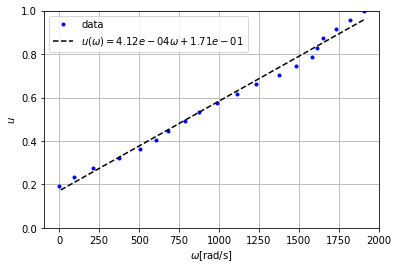
\includegraphics[width=13cm]{graficos/plot_test_calibration_result_feedforward.png}
    \caption{TESTE: RESULTADO DA IDENTIFICAÇÃO/CALIBRAÇÃO}
\end{figure}

\begin{figure}[H]
    \centering
    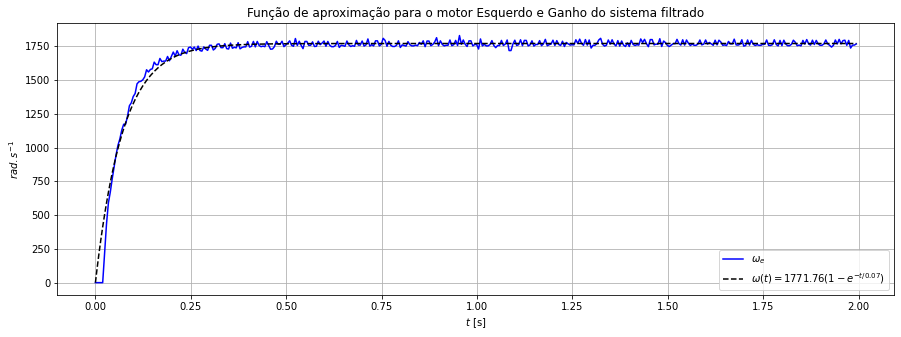
\includegraphics[width=13cm]{graficos/plot_test_identificacao.png}
    \caption{TESTE: RESULTADO DA IDENTIFICAÇÃO/CALIBRAÇÃO}
\end{figure}

\subsection{Filtragem da velocidade}
% MOSTRAR A FILTRAGEM COM DIFERENTES PARÂMETROS:
% sintonizando a incerteza da medição e do modelo (Q e R)

\begin{figure}[H]
    \centering
    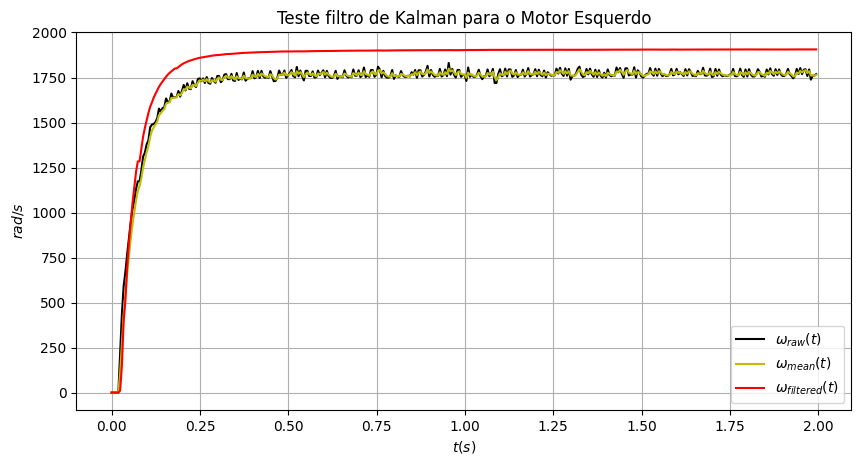
\includegraphics[width=13cm]{graficos/plot_test_media_x_kalman.png}
    \caption{TESTE: MEDIA VS KALMAN}
\end{figure}

\subsection{Respostas do sistema com os controladores}


\begin{figure}[H]
    \centering
    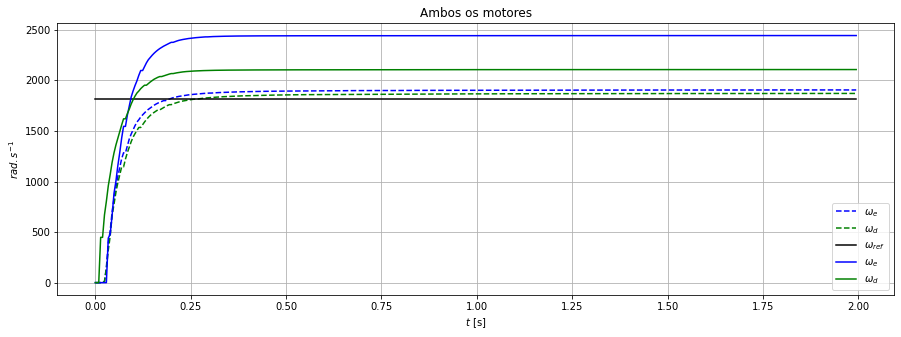
\includegraphics[width=13cm]{graficos/plot_test.png}
    \caption{TESTE: COM CONTROLE VS SEM CONTROLE}
\end{figure}

\begin{figure}[H]
    \centering
    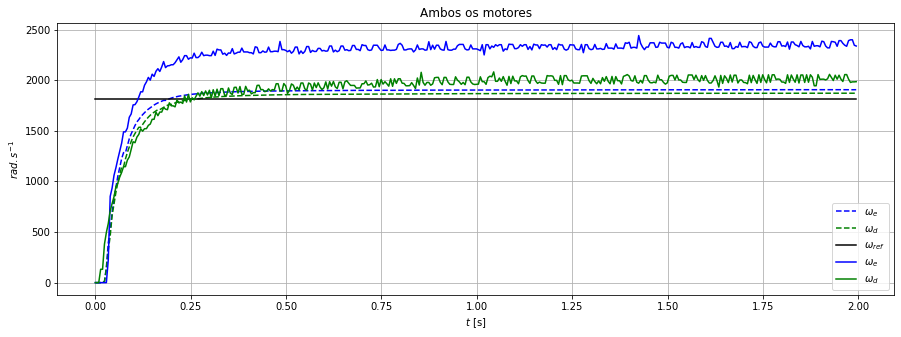
\includegraphics[width=13cm]{graficos/plot_test_antes_x_depois.png}
    \caption{TESTE: ANTES X DEPOIS}
\end{figure}
\section{CONCLUSÃO}

Lorem ipsum dolor sit amet, consectetur adipiscing elit. Fusce malesuada posuere viverra. In dignissim lacus at arcu tincidunt sollicitudin. Donec sed metus eget dui tincidunt faucibus. Vivamus eu turpis risus. Pellentesque sit amet consequat nibh. Fusce dignissim tortor suscipit ex elementum feugiat. Nullam blandit urna fermentum ante gravida, sed aliquam magna congue. Vivamus turpis eros, eleifend sed faucibus eget, ultrices ut ligula. In in iaculis massa. Orci varius natoque penatibus et magnis dis parturient montes, nascetur ridiculus mus. Suspendisse pretium consequat tristique. Vestibulum diam ligula, bibendum ut quam nec, hendrerit lobortis eros. Aliquam quis tellus eget felis laoreet tempor.

\bibliography{bibliografia}
\end{document}


